%% ============================================================================
%%  MA-CETSP follow-up paper — reviewed diagnostic manuscript
%%  Target: Expert Systems with Applications (Elsevier), cas-dc template
%%
%%  STATUS LEGEND used in comments below:
%%    [DATA]     marks a number or table whose source CSV is named in the comment
%%               beside it, so any figure can be traced back and regenerated.
%%    [VERIFY]   marks a claim to re-check against the run logs before submission.
%%
%%  Every number in this file is traceable to a CSV in the repository.
%%  Sources are given in comments next to each table.
%% ============================================================================

\documentclass[a4paper,fleqn]{cas-dc}

% APA 7 citations and references; compile the bibliography with Biber.
\usepackage[american]{babel}
\usepackage{csquotes}
\usepackage[backend=biber,style=apa,natbib=true]{biblatex}
\addbibresource{references.bib}
\AtBeginBibliography{\raggedright}
% Biber emits Unicode names; the CAS T1 font needs a TeX accent for g-breve.
\usepackage{newunicodechar}
\newunicodechar{ğ}{\u{g}}
\usepackage{amsmath,amssymb}
\usepackage{booktabs}
\usepackage{algorithm}
\usepackage{algpseudocode}
\usepackage{tikz}
\usetikzlibrary{arrows.meta,positioning,calc}

% ---------------------------------------------------------------------------
% Float placement.
%
% Symptom: on the first full build every \includegraphics figure was deferred
% past the bibliography while all ten tables placed correctly. In two-column
% LaTeX a deferred float forces every later float of its class to be deferred
% too, so one early failure cascades to the end of the document.
%
%   placeins  with [section] flushes pending floats at each \section, so a
%             figure cannot drift past the section that discusses it.
%
% NOTE: do NOT add dblfloatfix here. cas-dc.cls already loads stfloats (see its
% line 63), the two are mutually exclusive, and loading both aborts the build
% with "Command \c@dblbotnumber already defined". stfloats already provides what
% we need from it -- full-width floats may be placed at the BOTTOM of a page --
% which is why the starred floats below are declared [!tbp] rather than [!tp].
% ---------------------------------------------------------------------------
\usepackage[section]{placeins}

% Two-column pages are narrow; tighten inter-column padding so tables fit.
% One wide table (tab:model-comparison) uses table* and spans the full width.
\setlength{\tabcolsep}{4pt}
\setlength{\emergencystretch}{3em}

% graphicx is already loaded by cas-dc.cls; just point it at the figure folder.
% Figures are regenerated by analysis_la_cetsp/make_figures.py, which reads the
% result CSVs — rerun it after new measurements instead of editing them by hand.
\graphicspath{{figures/}}
% Generated by tools/export_paper_results.py
\newcommand{\KappaVNDMean}{0.889}
\newcommand{\KappaVNDMin}{0.664}
\newcommand{\KappaVNDMax}{0.951}
\newcommand{\ObservedRankC}{0.560}
\newcommand{\CalibrationStartC}{0.730}
\newcommand{\CalibrationEndC}{0.502}
\newcommand{\GreedyMin}{0.555}
\newcommand{\GreedyMax}{0.990}
\newcommand{\LkhRankMin}{0.516}
\newcommand{\LkhRankMax}{0.646}
\newcommand{\RefineMin}{0.416}
\newcommand{\RefineMax}{0.577}
\newcommand{\GlobalRankMin}{0.129}
\newcommand{\GlobalRankMax}{0.479}
\newcommand{\CohortRankMin}{0.080}
\newcommand{\CohortRankMax}{0.205}
\newcommand{\LkhCircle}{0.921}
\newcommand{\LkhKro}{0.944}
\newcommand{\LkhRat}{0.820}
\newcommand{\RejectionSpeedRho}{0.817}
\newcommand{\RejectionSpeedP}{0.007}


% ---------------------------------------------------------------------------
% Float placement. The default LaTeX parameters are conservative: at most two
% floats at the top of a page, and a page must be >=20% text before a float may
% be added. With 13 floats this pushes everything to the end of the document.
% Relaxed below to accommodate the manuscript's full-width figures and tables.
% ---------------------------------------------------------------------------
\setcounter{topnumber}{3}          % floats allowed at the top of a page
\setcounter{bottomnumber}{2}       % ... and at the bottom
\setcounter{totalnumber}{5}        % ... in total on one page
\renewcommand{\topfraction}{0.9}   % page may be 90% float at the top
\renewcommand{\bottomfraction}{0.7}
\renewcommand{\textfraction}{0.07} % a page needs only 7% text
\renewcommand{\floatpagefraction}{0.7}  % a float page must be 70% full
\setcounter{dbltopnumber}{3}            % same, for full-width (starred) floats
\renewcommand{\dbltopfraction}{0.9}
\renewcommand{\dblfloatpagefraction}{0.7}

\begin{document}
\let\WriteBookmarks\relax
% These two lines ship with the CAS template. Both names are misspellings of the
% real LaTeX parameters (\floatpagefraction and \textfraction) and are used
% nowhere in cas-dc.cls or cas-common.sty, so they have no effect. The genuine
% parameters are set in the preamble above; these are kept only to stay close to
% the distributed template.
\def\floatpagepagefraction{1}
\def\textpagefraction{.001}

% The running head is a fixed-width box; the full title overflows it by ~123pt
% and produces an Overfull \hbox at \maketitle. Keep this short.
\shorttitle{Pre-local-search surrogate filtering}
\shortauthors{D. Balemir and D. Cant{\"u}rk}

\title[mode=title]{Assessing the Viability of Pre-Local-Search Surrogate Filtering:
A Diagnostic Study of Survival-Based Offspring Pruning in Memetic CETSP}

\author[1]{Demir Balemir}[orcid=0009-0005-6589-9533]
\cormark[1]
\ead{demir.balemir@tedu.edu.tr}

\author[1]{Deniz Cant{\"u}rk}[orcid=0000-0002-7606-8701]
\ead{deniz.canturk@tedu.edu.tr}

\affiliation[1]{organization={Department of Computer Engineering, TED University},
                city={Ankara}, country={T\"urkiye}}

\cortext[1]{Corresponding author.}

% ============================================================================
% ABSTRACT
% ============================================================================
\begin{abstract}
Surrogate-assisted evolutionary computation substitutes cheap learned
predictions for expensive fitness evaluations. In memetic algorithms the
analogous idea is to filter offspring \emph{before} local search, since local
search dominates the per-iteration cost. We realise this idea in full for the
Close-Enough Traveling Salesman Problem (CETSP): offspring are described at
birth by geometric and cost features, labelled by their survival time in the
population, and scored by a survival model that gates variable-neighbourhood
descent (VND). Nine survival models run concurrently on parallel islands
alongside an in-run no-filter control. On 53 benchmark instances with five seeds
per configuration, we detect no statistically significant differences in solution
quality or convergence speed. Diagnostic analyses find limited discrimination
(cross-validated concordance $\approx 0.53$), with similar findings across the
tested model classes and feature families. An oracle using recorded post-VND
information reaches $0.687$, providing an empirical reference for prediction.
Stage-wise measurements show instance-dependent rank transmission through greedy,
Lin--Kernighan and refinement stages. Lower-ranked inputs tend to improve more.
These observations motivate a one-sided viability gate centred on three checks:
target predictability, rank transmission and discrimination beyond drift. The
diagnostics are conditional on recorded, admitted solutions. Adverse findings
can support reconsidering the tested design; favourable findings justify further
evaluation without establishing that filtering will pay off.

\end{abstract}

\begin{keywords}
Close-enough traveling salesman problem \sep Memetic algorithm \sep
Surrogate-assisted evolutionary computation \sep Survival analysis \sep
Local search \sep Viability assessment
\end{keywords}

\maketitle

% ============================================================================
\section{Introduction}\label{sec:intro}
% Paragraphs 1-4 carry over from the preliminary study almost verbatim; the
% contribution list (P5) and the results preview were rewritten for this paper.
% ============================================================================

% --- P1: problem definition -------------------------------------- [WRITTEN]
Given a set of $N$ targets $V=\{v_1,\dots,v_N\}$, each enclosed by a disk
neighbourhood $D_i$ of radius $r_i$, the Close-Enough Traveling Salesman Problem
(CETSP) asks for a minimum-cost closed tour passing through at least one point
of every disk. Unlike the classical TSP, only proximity is required: any
interior point of $D_i$ constitutes a valid visit. When all radii vanish the
problem reduces to the TSP, confirming NP-hardness. This spatial flexibility
makes the CETSP a natural model for autonomous routing where exact waypoint
precision is neither required nor achievable: UAV mission planning, robotic
infrastructure inspection, mobile data collection in wireless sensor networks,
and precision agriculture. These are not hypothetical settings: recent work
plans unmanned-aerial-vehicle trajectories directly as a
CETSP~\citep{cariou2023geometric}, schedules inspection flights over engineering
assets~\citep{zhen2024uavinspection}, and routes vessel-launched UAV swarms
across off-shore wind farms~\citep{ismail2025uavwind}, in each case exploiting
the fact that a target is served from anywhere within sensing range.

% --- P2: solution landscape -------------------------------------- [WRITTEN]
Early work addressed this difficulty through Steiner-zone constructions and
second-order cone programming (SOCP) reformulations, achieving provable
optimality on small instances at exponential runtime
cost~\citep{behdani2014integer,coutinho2016branch}; branch-and-bound methods
have since been refined further and now close benchmark instances that were
previously open~\citep{zhang2023cetspbb}. Discretisation-based
heuristics~\citep{CARRABS2017163,carrabs2020adaptive} extended tractability to
medium-sized problems, and a genetic algorithm with SOCP refinement later
reported 32 new best-known solutions on standard
benchmarks~\citep{DIPLACIDO2022105831}. The problem has also been generalised
along several axes (profits attached to targets~\citep{diplacido2023generalized},
multiple vehicles~\citep{carrabs2025upper}, and explicitly modelled service
times at each target~\citep{cui2026service}), which keeps the underlying
solvers under continuous pressure. More recently, nature-inspired
metaheuristics have been applied to the CETSP, including Harris Hawks
Optimisation~\citep{dokeroglu2025hho} and a parallel fitness-oriented memetic
algorithm~\citep{canturk2025parallel}. The current state of the art, MA-CETSP,
proposed by \citet{LEI2024111266}, combines a multi-step crossover (MSX)
operator with variable-neighbourhood descent (VND) local search inside a
diversity-preserving population-management framework, yielding 30 new best-known
solutions across 62 benchmark instances and establishing VND-based memetic
search as the dominant paradigm for large-scale CETSP; subsequent work has shown
that this paradigm scales further still when the population is distributed
across cores~\citep{canturk2026scalable}.

% --- P2b: the learning turn in optimisation ----------------------------- [NEW]
% Added at the reviewers' / editorial request for a fuller positioning of the
% work within current AI-assisted optimisation research.
A second line of development runs alongside this algorithmic one. Machine
learning has moved from a peripheral tool to a structural component of modern
optimisation, and recent surveys map the resulting design space in
detail~\citep{talbi2021mlmeta,bolufe2025mlmeta}: learned components now select
operators, tune parameters, control restarts and rank candidate solutions.
Within routing specifically, end-to-end neural solvers have matured into a
research area of their own~\citep{wu2026ncosurvey}, and the approach has already
reached the CETSP~\citep{fan2025ud3rl}. A parallel and more conservative strand
keeps a proven metaheuristic in place and inserts a learned decision at a single
point inside it: Q-learning selects among low-level heuristics in a selection
hyper-heuristic~\citep{zhao2023qlhh}, deep reinforcement learning does the same
under uncertainty~\citep{zhang2022drlhh}, a Q-learning controller governs the
local-search step of a memetic algorithm~\citep{zhang2024qlmemetic}, and a
learned model predicts which heuristic to run on a given
instance~\citep{karcher2025heuristic}. The appeal of this second strand is that
the solver's operators and tuning survive intact; what the learned component
changes is only how a fixed budget is spent.

% --- P2c: surrogate-assisted EC, and the gap this paper addresses -------- [NEW]
The specific form of learned decision that concerns us here is the
\emph{surrogate}: a cheap model consulted in place of an expensive evaluation.
Surrogate-assisted evolutionary computation is a mature field with its own
reviews and taxonomies~\citep{jin2005comprehensive,he2023review}, and its scope
now extends well past the continuous, low-dimensional problems where it began,
into combinatorial and permutation-based
search~\citep{liu2024combinatorial}, including memetic algorithms in which the
surrogate decides which individuals are worth
refining~\citep{nishihara2025memetic}. Two lessons from that literature bear
directly on what follows. First, a surrogate need not predict fitness
numerically: it is often sufficient, and empirically more robust, to learn a
classification or a pairwise relation among candidates and use it to admit or
reject them~\citep{li2022classification,hao2024unevaluated}. Second, surrogate
use must be managed rather than assumed beneficial, because an inaccurate model
biases the search instead of merely slowing it: approximation error acts like
noise injected into selection~\citep{zheng2024noise}, and the accuracy a
surrogate must attain before it helps at all has itself become an object of
study~\citep{hanawa2025impact}. This motivates a complementary question: whether
the information available before local search supports discrimination useful
for filtering. The present paper examines this question through measurements of
predictive performance and rank transmission in a memetic CETSP pipeline.

% --- P3: the inefficiency that motivates filtering ---------------- [WRITTEN]
Despite its strong empirical performance, MA-CETSP applies VND
to every generated offspring. Because VND dominates the per-iteration runtime,
evaluating offspring that will be discarded immediately consumes computation
that selective filtering might save. In a preliminary
study~\citep{balemir2026lacetsp} we augmented MA-CETSP with a
survival-analysis-based offspring filter and reported that 13--26\% of offspring
could be pruned on four benchmark instances while maintaining competitive
solution quality.

% --- P4: what that study could not settle ------------------------- [REWRITE]
% IMPORTANT: this paragraph must now do double duty — motivate the extension AND
% set up the self-correction. Do not hide that the preliminary result does not
% survive; a reviewer who reads both papers will find it.
The scope of that preliminary study limited the strength of its conclusions.
Four instances, five seeds and a 500-iteration budget offered limited evidence
for separating a filtering effect from run-to-run variation, and no concordance
index was reported for any model. The present work extends the evaluation and
finds no statistically detectable benefit at the larger scale. It also examines
the predictive and pipeline characteristics that may account for this outcome.

% --- P5: contributions ------------------------------------------------------
This paper makes four contributions.
\textbf{(i) A complete surrogate-filtering framework for memetic CETSP.}
Nine survival models (Cox PH, ElasticNet Cox, RSF, GBSA, DeepSurv, SSVM,
WeibullAFT, MTLR and a $k$-NN survival estimator) run concurrently on
independent islands alongside an in-run no-filter control island, with an
adaptive training trigger, validation-calibrated rejection thresholds and a
rolling rejection-rate cap. The implementation removes the cross-language
inference bottleneck identified as the main limitation of the preliminary study.
\textbf{(ii) A large-scale evaluation.} On 53 benchmark instances with five
seeds per configuration, we detect no statistically significant differences in
solution quality or convergence speed relative to the baseline.
\textbf{(iii) A diagnosis.} We document limited discrimination across the tested
model classes and feature families, and identify attenuation of cost ordering
through local search, particularly at the LKH stage, as a contributing mechanism.
\textbf{(iv) A viability gate.} We propose a low-cost, one-sided screening
procedure and apply it retrospectively to CETSP. It can support a decision
against a filtering design under the assessed conditions; passing it supports
further evaluation rather than establishing benefit.

% --- P6: roadmap ------------------------------------------------------------
Section~\ref{sec:related} surveys related work. Section~\ref{sec:framework}
describes the framework. Section~\ref{sec:setup} details the experimental setup.
Section~\ref{sec:results} reports the effect of filtering.
Section~\ref{sec:diagnosis} examines the observed outcome. Section~\ref{sec:gate}
derives the viability gate. Section~\ref{sec:discussion} discusses implications
and threats to validity, and Section~\ref{sec:conclusion} concludes.

% ============================================================================
\section{Related Work}\label{sec:related}
% ============================================================================

\subsection{Early and Exact Approaches}\label{sec:rel-exact}

The CETSP was formally defined by \citet{gulczynski2006close} as a geometric
relaxation of the classical TSP in which each target is enclosed by a circular
neighbourhood of radius $r_i$, and any interior point constitutes a valid visit.
Initial solution strategies combined supernode construction with
Steiner-zone-based local refinement to produce feasible tours. Exact
formulations based on Mixed-Integer Programming (MIP) and Second-Order Cone
Programming (SOCP) were later
developed~\citep{behdani2014integer,coutinho2016branch}, delivering provably
optimal solutions for small instances at the cost of exponential runtime growth
as problem size increases.

Carrabs et al.\ addressed this scalability limitation through adaptive
discretisation, transforming the continuous CETSP into a sequence of discrete
subproblems amenable to classical combinatorial
solvers~\citep{CARRABS2017163,carrabs2020adaptive}. The accompanying
variable-neighbourhood search heuristics achieved tighter bounds and faster
runtimes, establishing discretisation-based approaches as competitive
alternatives to exact methods.

Exact optimisation of the CETSP has remained active.
\citet{zhang2023cetspbb} present a branch-and-bound algorithm that resolves
benchmark instances left open by earlier exact work, and the problem has been
extended in several directions that keep the exact machinery under development:
a generalised variant in which targets carry
profits~\citep{diplacido2023generalized}, a multiple-vehicle formulation for
which upper-bounding procedures were recently
proposed~\citep{carrabs2025upper}, and a version in which the service time spent
at each target is modelled explicitly rather than assumed
negligible~\citep{cui2026service}. Exact methods nonetheless remain confined to
instance sizes well below those studied here, which is why heuristic search
retains its role.

\subsection{Metaheuristic and Hybrid Methods}\label{sec:rel-meta}

Population-based metaheuristics have become the dominant paradigm for
large-scale CETSP instances. \citet{DIPLACIDO2022105831} coupled a genetic
algorithm with SOCP-based refinement and 2-opt local search, reporting 32 new
best-known solutions on standard benchmarks and demonstrating that hybridising
evolutionary search with continuous optimisation yields highly competitive
outcomes.

The current state of the art is the Memetic Algorithm for CETSP (MA-CETSP)
proposed by \citet{LEI2024111266}, which combines a multi-step crossover (MSX)
operator with variable-neighbourhood descent (VND) local search inside a
diversity-preserving population-management framework. MA-CETSP produced 30 new
best-known solutions across 62 benchmark instances, surpassing all prior
methods. Despite its strong performance, the algorithm applies VND
to every generated offspring, motivating an assessment of whether selective
evaluation could reduce computational cost.
\citet{canturk2025parallel} subsequently introduced a parallel
fitness-oriented memetic algorithm that exploits multi-core architectures to
reduce wall-clock time, extended in \citet{canturk2026scalable} to substantially
larger instances by distributing the population across cores, and
\citet{derouiche2025deep} proposed deep crossover operators to enrich offspring
diversity in genetic search. Working from the geometry rather than the
population side, \citet{cariou2023geometric} combined an evolutionary algorithm
with heuristics tailored to the disk neighbourhoods themselves and applied the
result to unmanned-aerial-vehicle trajectory planning.

\subsection{Learning-Based Optimisation}\label{sec:rel-learning}

Machine learning has been integrated into combinatorial optimisation through two
principal paradigms, whose design space is catalogued in recent surveys of the
field~\citep{talbi2021mlmeta,bolufe2025mlmeta}. End-to-end deep reinforcement
learning (DRL) approaches, of which the Attention
Model~\citep{kool2019attention} is the canonical routing example, and which
\citet{wu2026ncosurvey} survey comprehensively for vehicle routing problems,
learn constructive policies for routing problems that achieve near-optimal
quality at inference speed. \citet{fan2025ud3rl} transferred this paradigm to
the CETSP through a Unified Dual-Decoder DRL framework combining a Transformer
encoder with $k$-nearest-neighbour subgraph reasoning. End-to-end learned solvers
provide an alternative to inserting learned decisions into an existing search
pipeline; the latter retains its established operators and instance-specific
tuning.

A complementary strategy retains a high-quality solver and applies learned
models selectively to reduce its computational burden. Selection
hyper-heuristics learn which low-level heuristic to apply next, using
Q-learning~\citep{zhao2023qlhh} or deep reinforcement learning under
uncertainty~\citep{zhang2022drlhh}; \citet{zhang2024qlmemetic} place a
Q-learning controller on the local-search step of a memetic algorithm; and
\citet{karcher2025heuristic} predict, per instance, which of several heuristics
will perform best. In each case the learned model redistributes a fixed
computational budget rather than replacing the search that consumes it. The
offspring filter studied in this paper belongs to this family, with one
distinction relevant to its assessment: it is asked to predict the outcome of the
transformation it is trying to avoid executing.

In our preliminary
study~\citep{balemir2026lacetsp} we introduced a learning-assisted extension of
MA-CETSP in which offspring are scored by a survival analysis model prior to
local search, allowing unpromising candidates to be discarded without VND
evaluation. On four benchmark instances, 13--26\% of offspring were pruned with
only marginal reported degradation in solution quality. That study did not,
however, report the discriminative power of any of the fitted models, and the
present work finds no statistically significant benefit in the larger evaluation
of Section~\ref{sec:results}.

\subsection{Surrogate-Assisted Evolutionary Computation}\label{sec:rel-surrogate}

The idea of substituting a cheap learned approximation for an expensive
evaluation is long established in evolutionary computation.
\citet{jin2005comprehensive} surveys fitness approximation in evolutionary
algorithms and establishes the design vocabulary still in use: the choice of
approximation model, the amount of true evaluation retained, and the burn-in
period required before a surrogate is trustworthy (typically 10--20\% of the
evaluation budget), a guideline we adopt directly in
Section~\ref{sec:fw-trigger}. \citet{jin2011surrogate} reviews subsequent
advances and identifies the central open difficulty: a surrogate that is
inaccurate in the region the search is currently exploring can actively mislead
the population toward false optima, so surrogate use must be managed rather than
assumed beneficial. This concern gave rise to the literature on
\emph{evolution control} and \emph{model management}, which regulates how often
the true objective is consulted; \citet{he2023review} review the resulting body
of work and the model-management strategies it has produced. Two recent results
sharpen the point. \citet{zheng2024noise} show that surrogate approximation
error is usefully treated as noise injected into selection, rather than as a
uniform loss of precision, and \citet{hanawa2025impact} study directly how
accurate a surrogate must be before it improves search at all, finding that the
appropriate model-management strategy itself depends on that accuracy. Both
motivate examining whether the available inputs support sufficient predictive
accuracy for a particular filtering decision, the question studied here.

Within memetic algorithms specifically, surrogates have been applied not only to
approximate fitness but to decide \emph{where} local search should be invoked.
\citet{lim2010generalizing} generalise surrogate-assisted memetic computation
and show that ensembles and locally weighted models can identify individuals
that warrant refinement, concentrating an expensive improvement operator on the
most promising regions of the search space. The offspring filter studied in this
paper belongs squarely to that family: the surrogate does not replace the
objective, it gates access to the local search.

Two further developments make that family directly relevant to the CETSP.
First, surrogate assistance is no longer confined to continuous decision
spaces: \citet{liu2024combinatorial} survey surrogate-assisted evolutionary
algorithms for expensive \emph{combinatorial} optimisation, and
\citet{nishihara2025memetic} build a surrogate-assisted memetic algorithm for
permutation-based problems in which a discrete-space surrogate decides where the
expensive operator is applied, structurally the closest existing analogue to
the filter evaluated here. Second, the surrogate's target need not be a fitness
value. Classification-based surrogates learn only whether a candidate is good or
poor~\citep{li2022classification}, and relation-based surrogates learn a
pairwise comparison between candidates and use it to admit unevaluated solutions
into the population~\citep{hao2024unevaluated}; both are natural fits for an
accept/reject gate and need not reconstruct exact fitness values.
Alongside these, work on composite and ensemble
surrogates~\citep{zhai2024composite} and on using explainability to accelerate
surrogate-assisted search~\citep{li2024explainable} illustrates how much design
effort the field currently invests in improving surrogate quality. Section
\ref{sec:diagnosis} complements these approaches by examining limitations of
the tested inputs and target before further model development is considered.

Two features of the established evaluation practice in this literature motivate
the present study. First, surrogates are predominantly assessed by their effect
on end-to-end search performance, which conflates the quality of the surrogate
with the robustness of the search to a poor one; the standalone discriminative
power of the fitted model is reported comparatively rarely. Second, and more
consequentially, the transformation that sits \emph{between} the surrogate's
inputs and its target is seldom examined. In a memetic algorithm that
transformation is the local search itself. Attenuation of the entering cost
ordering may limit the usefulness of cost-based pre-local-search descriptors,
although it does not exclude predictive information in other representations.
To our knowledge this rank-transmission question has not been posed as an
explicit diagnostic for surrogate-assisted filtering. Providing such a measure
and assessing it alongside predictive performance is the contribution of this
paper.

\subsection{Survival Analysis Methods}\label{sec:rel-survival}

Survival analysis models the time until an event of interest and naturally
accommodates censored observations. Cox Proportional Hazards (Cox
PH)~\citep{cox1972regression} is the canonical semi-parametric baseline,
estimating a log-linear hazard as a linear function of covariates; an
elastic-net-penalised variant~\citep{simon2011regularization} extends it to
correlated or high-dimensional feature spaces. Random Survival Forests
(RSF)~\citep{ishwaran2008random} aggregate survival trees grown on bootstrap
samples to capture non-linear covariate interactions, while Gradient Boosting
Survival Analysis (GBSA)~\citep{hothorn2006survival} optimises a Cox
partial-likelihood loss stagewise, producing sharper decision boundaries.
DeepSurv~\citep{katzman2018deepsurv} replaces the linear Cox predictor with a
deep neural network to model complex non-linear hazard landscapes, and
MTLR~\citep{yu2011learning} discretises the time axis and learns a sequence of
logistic regressors, implemented here via a neural-network backbone. Survival
Support Vector Machines (SSVM)~\citep{van2007support} cast the ranking problem
induced by censored data as a structured SVM objective, whereas the Weibull
Accelerated Failure Time model (WeibullAFT)~\citep{wei1992accelerated} directly
regresses log-survival time under a parametric distributional assumption.
Finally, a $k$-NN survival estimator assigns risk scores as the negative mean
survival time of the $k$ nearest training neighbours~\citep{pedregosa2011scikit},
serving as a non-parametric baseline. Together, these nine models span the
spectrum from interpretable parametric methods to flexible deep learners,
enabling a systematic comparison of pruning behaviour across diverse modelling
assumptions.

The choice to span the spectrum rather than to select a single model is
deliberate, and is supported by the current state of the survival-analysis
literature. \citet{wiegrebe2024dlsurvival} review deep learning for survival
analysis and find a field in which architectural variety has grown much faster
than evidence of consistent superiority, and \citet{burk2026neutral} report a
large-scale neutral comparison in which no model class dominates on
low-dimensional data: classical Cox-type models remain competitive with
tree-based and neural alternatives. We therefore treat the nine models as a
sensitivity analysis over modelling assumptions rather than as a ranking
exercise, and Section~\ref{sec:diag-cindex} interprets their concordance indices
in that spirit.

% ============================================================================
\section{Framework}\label{sec:framework}
% Target ~8-10 manuscript pages. All material exists in the codebase.
% ============================================================================

Figure~\ref{fig:architecture} gives the system in one view and
Algorithm~\ref{alg:main} states it precisely; this section explains each part
and the reasoning behind it.

% Declared here, immediately after its first citation, NOT at the end of the
% section. A float cannot be placed before the point it is declared, so with
% the declaration at the end of Section 3 this full-width figure could never
% reach the pages that discuss it; it was then flushed by the placeins
% barrier at Section 4 and left the preceding page half empty.
% NOTE: seven boxes across is close to \textwidth. If this overflows on your
% build, wrap the tikzpicture in \resizebox{\textwidth}{!}{...} or drop the
% node distance to 3mm — do not shrink the fonts further.
\begin{figure*}[!tbp]
\centering
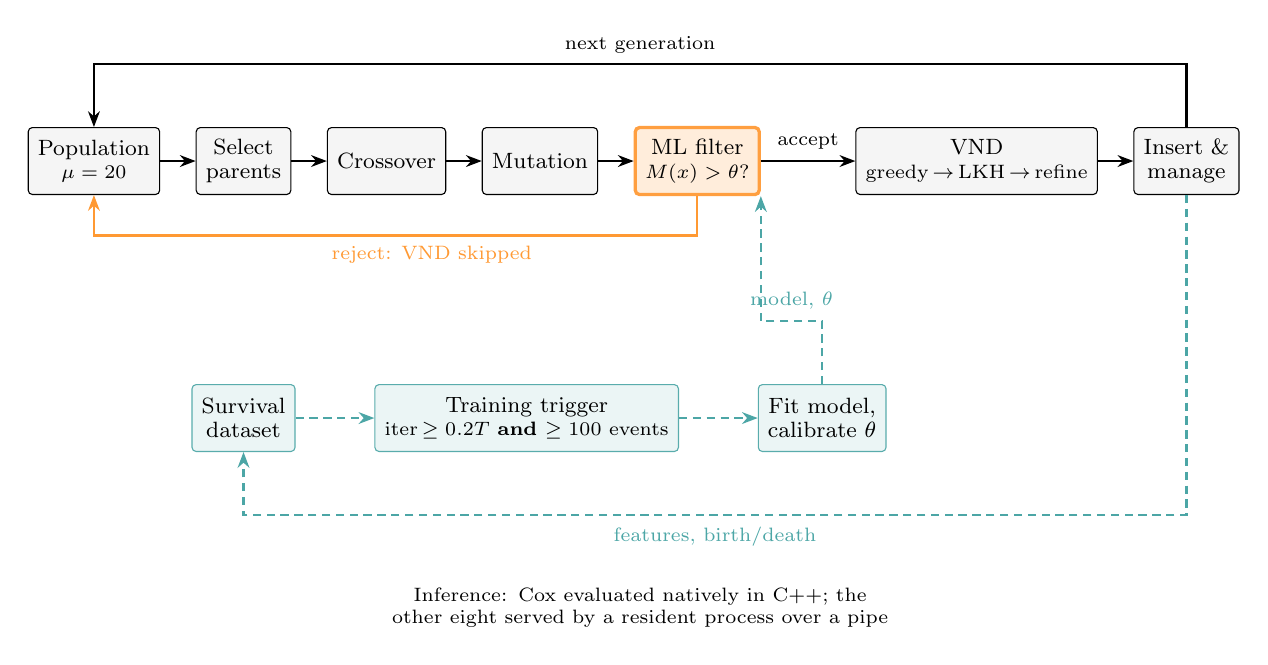
\begin{tikzpicture}[
  >={Stealth[length=2mm]},
  node distance=4.5mm,
  box/.style={draw, rounded corners=1.5pt, align=center, font=\footnotesize,
              minimum height=8.5mm, inner xsep=3.5pt},
  op/.style={box, fill=black!4},
  ml/.style={box, fill=teal!8, draw=teal!65},
  filt/.style={box, fill=orange!14, draw=orange!75, very thick},
  flow/.style={->, thick},
  data/.style={->, densely dashed, teal!70, thick},
]
% ---- search loop (top row) -------------------------------------------------
\node[op] (pop) {Population\\[-1pt]{\scriptsize $\mu=20$}};
\node[op,  right=of pop]  (par)  {Select\\[-1pt]parents};
\node[op,  right=of par]  (xo)   {Crossover};
\node[op,  right=of xo]   (mut)  {Mutation};
\node[filt,right=of mut]  (filt) {ML filter\\[-1pt]{\scriptsize $M(x)>\theta$?}};
\node[op,  right=12mm of filt] (vnd)  {VND\\[-1pt]{\scriptsize greedy\,$\to$\,LKH\,$\to$\,refine}};
\node[op,  right=of vnd]  (ins)  {Insert \&\\[-1pt]manage};

\foreach \a/\b in {pop/par, par/xo, xo/mut, mut/filt, vnd/ins}
  \draw[flow] (\a) -- (\b);

% The wider gap fits the label directly above the accepting arrow.
\draw[flow] (filt.east) -- node[above=1mm, font=\scriptsize, inner sep=1pt]
      {accept} (vnd.west);

% return of the surviving population
\draw[flow] (ins.north) -- ++(0,8mm) -| node[pos=0.25, above, font=\scriptsize]
      {next generation} (pop.north);

% rejection bypasses the expensive stage entirely
\draw[flow, orange!80] (filt.south) -- ++(0,-5mm)
      -| node[pos=0.22, below, font=\scriptsize] {reject: VND skipped} (pop.south);

% ---- learning loop (bottom row) --------------------------------------------
% Start the learning row on the left, leaving the right edge clear for logging.
\node[ml, below=24mm of par] (ds) {Survival\\[-1pt]dataset};
\node[ml, right=10mm of ds] (trig)
     {Training trigger\\[-1pt]{\scriptsize iter\,$\geq0.2T$ \textbf{and} $\geq100$ events}};
\node[ml, right=10mm of trig] (fit) {Fit model,\\[-1pt]calibrate $\theta$};

\draw[data] (ds)   -- (trig);
\draw[data] (trig) -- (fit);

% Route logging below the learning row, then enter the dataset from below.
% This keeps the return path out of the boxes and the two learning arrows.
\coordinate (loglane) at ($(ds.south)+(0,-8mm)$);
\draw[data] (ins.south) -- (ins.south |- loglane)
      -- node[midway, below=1mm, font=\scriptsize, inner sep=1pt]
         {features, birth/death} (loglane)
      -- (ds.south);

% the fitted model and its threshold arm the filter -- this closes the cycle
\coordinate (modellane) at ($(fit.north)+(0,8mm)$);
\draw[data] (fit.north) -- (modellane)
      -- node[midway, above=1mm, font=\scriptsize, inner sep=1pt]
         {model, $\theta$} (filt.south east |- modellane)
      -- (filt.south east);

% ---- inference paths -------------------------------------------------------
\coordinate (diagrammid) at ($(pop.center)!0.5!(ins.center)$);
\node[font=\scriptsize, align=center, text width=0.92\textwidth,
      anchor=north, yshift=-8mm] at (diagrammid |- loglane)
      {Inference: Cox evaluated natively in C++; the other eight
       served by a resident process over a pipe};
\end{tikzpicture}
\caption{The filtered memetic algorithm. The search loop (solid) is the baseline
of Section~\ref{sec:fw-baseline} with one insertion: the filter sits between
mutation and local search, the only position at which a rejection saves the cost
it is meant to save. The learning loop (dashed) closes the cycle: the search
generates its own training data, a model is fitted once the trigger conditions of
Equations~\eqref{eq:trig-budget}--\eqref{eq:trig-events} are met, and the
calibrated threshold arms the filter for the remainder of the run. A rejected
offspring bypasses VND entirely and is neutral for the stagnation counter.}
\label{fig:architecture}
\end{figure*}

\subsection{Baseline: MA-CETSP}\label{sec:fw-baseline}

Our baseline is the memetic algorithm of \citet{LEI2024111266}, and we describe
it only to the depth the rest of the paper depends upon.

A population $P$ of $\mu = 20$ tours is initialised by $k$-means clustering of
the target disks, followed by an LKH pass and a greedy geometric adjustment on
each member. Every iteration draws two parents uniformly, produces one offspring
by the $k$-step crossover operator, applies a mutation with probability
proportional to the current stagnation counter, and passes the offspring to
variable-neighbourhood descent. Two properties of this loop matter downstream.

\textbf{Local search dominates the cost, and it is a pipeline.} The VND stage is
not a single operator but a sequence: a cheap greedy repositioning of the visit
points, an LKH solve on the induced tour, a second greedy pass, a
best-improvement relocate-and-swap over a 50-neighbour candidate list, and a
final continuous refinement of the visit points. The LKH solve dominates the
runtime, and it is this internal structure that Section~\ref{sec:diag-stages}
exploits to localise where information is lost.

\textbf{Survival is decided by rank, against the current population.} After each
insertion, every member is assigned
\begin{equation}
f(s) \;=\; \alpha \cdot r_{\text{val}}(s) \;+\; \beta \cdot r_{\text{div}}(s),
\qquad \alpha = 1,\; \beta = 0.96,
\label{eq:fitness}
\end{equation}
where $r_{\text{val}}$ is the rank of $s$ by tour cost and $r_{\text{div}}$ its
rank by minimum edit distance to the rest of the population, both scaled to
$[0, 100]$. When the population reaches $1.5\mu$ members it is sorted by $f$ and
truncated back to $\mu$. Equation~\eqref{eq:fitness} is what makes ``survival''
a well-defined label, and equally what makes it a moving target: both ranks are
relative to a population that keeps changing, so an individual's fate depends on
solutions that do not exist when it is evaluated. Section~\ref{sec:diag-oracle}
returns to this.

An offspring is admitted to the population if it either improves on the
incumbent best while differing from every member, or lies at edit distance
greater than five from its nearest neighbour in $P$; the diversity term in
Equation~\eqref{eq:fitness} then governs how long it stays.

\subsection{Offspring Survival as a Learning Problem}\label{sec:fw-survival}

Pre-local-search descriptors are stored on each evaluated offspring. Admitted
individuals are written to the log when evicted, yielding a birth iteration $b$,
death iteration $d$ and duration $t=d-b$. At the ML training trigger, surviving
admitted individuals are written as right-censored observations. Unadmitted
offspring and terminal survivors on the control island are not written to the
historical logs.

Survival analysis accommodates event times and censoring in the training data.
However, the offline diagnostics retain positive-lifetime records, excluding
immediate evictions as well as unlogged candidates and terminal survivors. The
absence of censored records in the control sample therefore reflects selection
into the recorded data, not complete observation of all lifetimes. All survival
and reconstructed-cohort diagnostics below are conditional on this sample.
Assessing predictability across all generated offspring requires complete
logging and new experiments.

\subsection{Feature Representation}\label{sec:fw-features}

Each individual is described at birth by ten quantities computed from the
pre-VND tour: the mean and variance of its edge lengths; the width, height and
area of its axis-aligned bounding box; the two coordinates of its centroid; the
sum of point-to-centroid distances; the variance of the turning angles at
interior vertices; and the pre-VND tour cost. This is the representation
inherited from the preliminary study, and it is the one actually deployed.

Two of its properties deserve to be stated here rather than discovered later.
Six of the ten (the three bounding-box quantities, the two centroid
coordinates and the centroid distance sum) are near-constant within an
instance, because every candidate tour visits the same set of disks and
therefore occupies almost the same region of the plane; they vary across
instances but barely within one, which is the only variation a per-instance
model can use. The implemented mean edge length omits the closing edge, so it is closely
related to tour cost but not exactly proportional to it. Section~\ref{sec:diag-features} quantifies the
consequences and tests four alternative representations.

\subsection{Survival Models}\label{sec:fw-models}

Nine models are integrated, chosen to span the modelling spectrum rather than to
represent a tuned selection. \emph{Cox proportional hazards} provides the
interpretable semi-parametric baseline, with an \emph{elastic-net penalised}
variant for the collinearity noted above. \emph{Random survival forests} and
\emph{gradient boosting survival analysis} capture non-linear interactions by
ensembling survival trees, the former by bagging and the latter by stagewise
optimisation of the Cox partial likelihood. \emph{DeepSurv} replaces the linear
predictor with a multilayer network, and \emph{MTLR} discretises the time axis
and learns a sequence of logistic models over it; both use a two-hidden-layer
network of 64 units with batch normalisation and dropout. \emph{Survival support
vector machines} treat the censored comparisons as a ranking problem, the
\emph{Weibull accelerated failure time} model imposes a parametric duration
distribution, and a \emph{$k$-nearest-neighbour} estimator scores an individual
by the negated mean survival of its fifteen nearest training neighbours, serving
as a non-parametric reference.

Each model exposes the same interface: fitted on the logged features and
durations, it returns a scalar risk score in which larger values indicate
shorter expected survival. The filter compares that score against a calibrated
threshold (Section~\ref{sec:fw-threshold}) and rejects the offspring when it is
exceeded.

\subsection{Parallel Architecture and the In-Run Control}\label{sec:fw-islands}

A run launches ten independent searches on one machine, one per thread. Nine
carry one survival model each; the tenth runs with filtering disabled and serves
as a control. Island $i$ is seeded with $\sigma + i$ for a run-level seed
$\sigma$, and each maintains its own population, log directory, model directory
and solver scratch space.

We are deliberate about what this is and is not. There is \textbf{no migration}
between the islands: no individual, no statistic and no model is exchanged. This
is therefore a parallel portfolio with a built-in ablation control, not an island
model in the sense the term normally carries in evolutionary computation, and we
avoid claiming otherwise. Its purpose is experimental rather than algorithmic
(it places all nine treatments and the control in the same run, on the same
machine, under the same load), and the reported per-run best is taken over the
control alone unless stated otherwise.

The seeding scheme has a consequence we carry into
Section~\ref{sec:disc-threats}: because island $i$ uses seed $\sigma + i$, a
model and the control never share a random stream, so model-versus-control
comparisons are unpaired at the seed level and aggregation over instances is
what recovers statistical power.

\subsection{Adaptive Training Trigger}\label{sec:fw-trigger}

The preliminary study trained at a fixed iteration, which allocates the same
burn-in to an instance that converges in two hundred generations and one that
improves for five thousand. We replace it with a trigger that fires once per
run, when both of the following hold:
\begin{align}
\text{iter} &\;\geq\; 0.20 \cdot \text{budget}, \label{eq:trig-budget}\\
\#\{\text{observed evictions}\} &\;\geq\; 100. \label{eq:trig-events}
\end{align}
A hard fallback at $0.50 \cdot \text{budget}$ fires regardless of
Equation~\eqref{eq:trig-events}, so a population that evicts rarely is never
postponed indefinitely.

The two conditions have different rationales. Equation~\eqref{eq:trig-budget} is
a burn-in: surrogate-assisted evolutionary computation conventionally withholds
the surrogate for the first 10--20\% of the evaluation budget so that it is
fitted on a population representative of the region being
searched~\citep{jin2005comprehensive,lim2010generalizing}.
Equation~\eqref{eq:trig-events} is a sample-size floor. Survival models are
constrained by the number of \emph{events}, not observations, and the
events-per-variable heuristic asks for roughly ten events per
covariate~\citep{peduzzi1995importance}; with ten covariates this gives one
hundred. More detailed sample-size considerations are discussed
by~\citet{riley2019minimum}. This is an operational training floor, not a
guarantee of adequate sample size for every model. The islands share trigger
conditions; their realised event counts and training sets may differ.

One design decision here is easy to get wrong and worth stating explicitly. The
trigger does \emph{not} consult the stagnation counter, and never resets it. The
counter drives both the mutation rate and the stopping rule, and it must advance
identically on the control and on every ML island for the comparison to mean
anything; an earlier arrangement in which training reset it gave the ML islands
a longer search and a lower mutation rate, which confounded exactly the
measurement the experiment exists to make.

\subsection{Threshold Calibration}\label{sec:fw-threshold}

A risk score becomes a filter only once a rejection threshold is chosen, and a
fixed percentile ignores both instance difficulty and model quality. We select
it on a held-out 20\% validation split which the model has not been fitted on.

For each candidate percentile $p \in \{50, 55, \dots, 95\}$ we compute the
implied rejection rate $r$ and the normalised survival gap
\begin{equation}
g \;=\; \frac{\bar{t}_{\text{accepted}} - \bar{t}_{\text{rejected}}}
              {\bar{t}_{\text{all}}},
\end{equation}
which is positive when accepted individuals do outlive rejected ones, and
maximise
\begin{equation}
J(r, g) \;=\; g \cdot \min\!\left(1, \tfrac{r}{r^{*}}\right)
              \;-\; \lambda \max(0,\, r - r^{*}),
\label{eq:softcap}
\end{equation}
with a target rejection rate $r^{*} = 0.20$ and a penalty weight $\lambda = 2$.

The shape of Equation~\eqref{eq:softcap} is a correction to the obvious choice.
Maximising $r \cdot g$ appears to balance pruning against discrimination, but on
a validation split the rejection rate is mechanically $(100 - p)/100$, so that
objective contains a built-in pull toward low percentiles that has nothing to do
with the model. The ramp term instead grants full credit for discrimination once
a target rejection rate is reached, and the penalty term discourages exceeding
it. Percentile candidates are not restricted, only the resulting rate is softly
capped, so models whose risk distributions require a low percentile retain
access to one.

\subsection{Rolling Rejection-Rate Cap}\label{sec:fw-cap}

A threshold calibrated on the training distribution can become miscalibrated
later in the run, since the offspring generated after the model is fitted are
drawn from a population the model never saw. Left unchecked this produced
rejection rates above 40\% on some seeds, collapsing diversity and stalling the
search.

We therefore add a runtime guard. Every 50 filter-eligible offspring the
realised rejection rate over the window is measured; if it exceeds 30\%, the
filter is suspended for the following window and the check repeats. The guard is
a safety mechanism rather than a tuning device, and Section~\ref{sec:results}
reports rejection rates well below the cap.

\subsection{Implementation}\label{sec:fw-impl}

The preliminary study named cross-language inference latency as the obstacle to
converting pruning into wall-clock savings: each prediction opened a fresh Python
process, and the overhead was comparable to the local-search call it was meant to
avoid. Two changes remove it.

Eight of the nine models are served by a \emph{resident} scoring process started
once per island and held open for the duration of the run, communicating over an
inherited pipe pair: the solver writes one JSON line and reads one score back,
so a prediction costs a round trip rather than an interpreter start-up. The
process is restarted only when the model is refitted, and is respawned
automatically if it dies. The Cox model bypasses the boundary entirely: its
coefficients and standardisation statistics are read from disk and the linear
predictor is evaluated natively, so Cox islands invoke no external process at
all.

Algorithm~\ref{alg:main} states the resulting loop. Two details in it are easy to
overlook. The filter is placed after mutation and before local search, which is
the only position at which a rejection saves the cost it is meant to save. And a
rejected iteration is treated as \emph{neutral} for stagnation: it neither resets
the counter nor advances it. An offspring that never reached local search is not
evidence that the search has converged, and counting it as such would let an
aggressive filter trigger a premature stop and then report the resulting short
run as a speed-up.

\begin{algorithm}[htbp]
\caption{One island of the filtered memetic algorithm}
\label{alg:main}
\begin{algorithmic}[1]
\Require instance $I$, budget $T$, patience threshold $\rho$, model $M$
\State $P \gets \textsc{Initialise}(I)$; \; $s^{*} \gets \textsc{Best}(P)$
\State $\pi \gets 0$; \; trained $\gets$ \textbf{false}
\For{$\text{iter} = 1 \dots T$}
  \State $s_a, s_b \gets \textsc{SelectParents}(P)$
  \State $s \gets \textsc{Crossover}(s_a, s_b)$
  \State \textbf{if} $\textsc{Rand}(1000) < \pi$ \textbf{then}
         $s \gets \textsc{Mutate}(s)$
  \State $\textit{rejected} \gets \textbf{false}$
  \If{trained \textbf{and} \textbf{not} suspended}
    \State $x \gets \textsc{Features}(s)$
    \Comment{pre-VND, no local search yet}
    \If{$M(x) > \theta$}
      \State $\textit{rejected} \gets \textbf{true}$
      \Comment{skip VND entirely}
    \EndIf
  \EndIf
  \If{\textbf{not} \textit{rejected}}
    \State $s \gets \textsc{VND}(s)$
    \Comment{dominant cost}
    \State $P \gets \textsc{Insert}(P, s)$; \;
           $\textsc{Manage}(P)$
    \Comment{Eq.~\eqref{eq:fitness}}
  \EndIf
  \If{$\textsc{Best}(P) < s^{*}$}
    \State $s^{*} \gets \textsc{Best}(P)$; \; $\pi \gets 0$
  \ElsIf{\textbf{not} \textit{rejected}}
    \State $\pi \gets \pi + 1$
    \Comment{rejections are neutral}
  \EndIf
  \State \textbf{if} trigger fires (Eqs.~\eqref{eq:trig-budget}--\eqref{eq:trig-events})
         \textbf{then} fit $M$, calibrate $\theta$, trained $\gets$ \textbf{true}
  \State \textbf{if} $\pi \geq \rho$ \textbf{then break}
\EndFor
\State \Return $s^{*}$
\end{algorithmic}
\end{algorithm}


% ============================================================================
\section{Experimental Setup}\label{sec:setup}
% ============================================================================

% [DATA] *** VERIFY THESE NUMBERS AGAINST THE RUN LOGS BEFORE SUBMISSION ***
% What the repository supports: 53 test instances, 5 seeds, 5000 iterations,
% 10 islands per run (analysis_test/results/model_comparison_full.csv reports
% n_instances = 53; run_experiment.ps1 defines 5 seeds). A separate 15-instance
% development set was run at 1000 iterations. The earlier draft stated
% "68 instances, 1000 iterations, ten seeds", which matches neither.

\subsection{Benchmark Instances}\label{sec:setup-instances}

We use the 68 CETSP instances established by prior work: overlap-ratio families
derived from TSPLIB problems, arbitrary-radius variants, structured synthetic
families and industrial car-door welding instances, with up to one thousand
targets. A 15-instance development set informed the framework design. The
remaining 53 instances form the end-to-end test set reported in
Section~\ref{sec:results} (Table~\ref{tab:instances}).

The retrospective diagnostics in Sections~\ref{sec:diagnosis}--\ref{sec:gate}
use separate subsets of available logs. The five-instance model and oracle subset
includes one development instance (\texttt{bonus1000}); the 25-instance VND
calibration includes eight development instances. These are exploratory
diagnostics, not an independent test of the gate. The released instance manifest
records every membership. The instrumented stage analyses use island-0 records;
model, oracle, lineage and full-VND calibration use island-9 records.

\begin{table}[htbp]
\caption{Test-set composition. Groups follow the standard naming: \texttt{or2},
\texttt{or10} and \texttt{or30} denote overlap ratios of 0.02, 0.1 and 0.3;
\texttt{rdmRad} denotes arbitrary radii; \texttt{real\_world} are the car-door
instances. ``Filter active'' counts instances on which at least one ML island
reached the training trigger.}
\label{tab:instances}
\centering\small
\begin{tabular}{lrr}
\toprule
Group & Instances & Filter active \\
\midrule
varied      & 22 & 19 \\
rdmRad      & 11 &  8 \\
or2         &  6 &  6 \\
or30        &  6 &  6 \\
or10        &  5 &  5 \\
real\_world &  3 &  3 \\
\midrule
\textbf{Total} & \textbf{53} & \textbf{47} \\
\bottomrule
\end{tabular}
\end{table}

\subsection{Protocol and Parameters}\label{sec:setup-protocol}

Every configuration uses five base seeds: $1$, $11$, $21$, $31$ and $41$.
Each run has ten islands
and an iteration budget of $T = 5000$, giving 265 runs of ten islands each, or
2650 island-runs in total. Search parameters follow the baseline: population
$\mu = 20$, diversity coefficient $\beta = 0.96$, insertion distance threshold
$5$, candidate neighbourhood size $50$, $k$-means initialisation, $k$-step
crossover, and edit distance as the population distance measure.

Early stopping fires after $\rho = \max(T/10, 50) = 500$ consecutive
non-improving iterations. The rule is identical on the control and on all nine
ML islands, and, as described in Section~\ref{sec:fw-trigger}, is never
touched by the training trigger. Consequently the budget is adaptive in
practice: instances that converge quickly stop early, and the median run
terminates near iteration $1400$ rather than exhausting the $5000$ available.
Filter-specific constants are those given in Section~\ref{sec:framework}: burn-in
$0.20T$, event floor $100$, hard fallback $0.50T$, target rejection rate $0.20$,
and a rolling cap of $30\%$ over windows of $50$ filter-eligible offspring.

All experiments were run on a single machine, specified in
Table~\ref{tab:environment}. Two details of it bear on the results. The ten
islands of a run execute concurrently as threads of one process, which fits
within the 14 physical cores, but they still contend for memory bandwidth and
for the LKH subprocesses each of them spawns; this is the concrete basis for
the timing caveat in Section~\ref{sec:setup-measures}. And although the machine
has a discrete GPU, the installed \texttt{PyTorch} build is CPU-only and CUDA was
unavailable, so DeepSurv and MTLR were fitted and evaluated on the CPU like every
other model. No model in this study received hardware acceleration that the
others did not.

CPU execution matches the evaluated workload: ten independent searches, a
dominant LKH stage, and models fitted once per run on roughly one thousand rows
of ten features. Inference scores one offspring at a time before the next search
step proceeds, making per-request latency relevant
(Section~\ref{sec:fw-impl}). GPU execution was not benchmarked, so the reported
timing comparisons apply to the CPU configuration.

\begin{table}[htbp]
\caption{Execution environment. All reported runs were produced on this
configuration.}
\label{tab:environment}
\centering\small
\begin{tabular}{ll}
\toprule
CPU      & Intel Core i7-12700H \\
         & 14C / 20T, 2.7\,GHz \\
         & L2 11.5\,MB, L3 24\,MB \\
Memory   & 32\,GB DDR4-3200 \\
Storage  & NVMe SSD \\
GPU      & unused (CPU-only build) \\
OS       & Windows 11 Pro (26200) \\
\midrule
Solver   & C++17, MSVC 2022, \texttt{/O2} \\
Build    & CMake 4.2 \\
LKH      & 2.0.11 \\
\midrule
Python   & 3.10.9 \\
         & scikit-survival 0.25.0 \\
         & lifelines 0.30.0 \\
         & scikit-learn 1.7.2 \\
         & PyTorch 2.11 (CPU) \\
         & pycox 0.3.0 \\
\bottomrule
\end{tabular}
\end{table}

\subsection{Evaluation Measures}\label{sec:setup-measures}

For each instance we report mean best cost over five runs, rejection counts and
total wall-clock runtime including training. Table~\ref{tab:model-comparison}
averages run-level ratios: degradation is $100(f_{mi}/f_{0i}-1)$ and speedup is
$t_{0i}/t_{mi}$, matched by instance and run identifier. The matches have distinct
random seeds because island $i$ uses $\sigma+i$. The ratio of mean costs is
generally different from the mean of these ratios.

Two-sided Wilcoxon signed-rank tests (normal approximation, no continuity
correction) use model-minus-control per-instance mean
differences, assuming symmetry of the difference distribution. Quality tests
use all 53 instances; runtime tests use the 47 instances with at least one
recorded rejection. Differences are rounded to ten decimal places before testing to avoid floating-point rank artefacts.

Ten islands share a machine, so runtimes include resource contention. Rejected
iterations skip VND and are neutral for the stagnation counter. Consequently,
iterations do not represent a fixed computational budget across treatments.
Runtime to the stopping rule is not time to a common target quality. No
compute-weighted speedup is reported: per-offspring VND timings were not logged.

% ============================================================================
\section{Effect of Survival-Based Filtering}\label{sec:results}
% ============================================================================

% [DATA] source: analysis_test/results/model_comparison_full.csv
\begin{table*}[!tbp]
\caption{Effect of each survival model relative to the in-run no-filter control,
over 53 test instances $\times$ 5 seeds. Degradation averages matched run-level cost ratios;
positive means worse. No difference is statistically significant
($p \geq 0.31$ for quality, $p \geq 0.15$ for speed).}
\label{tab:model-comparison}
\centering\small
\begin{tabular}{lrrrr}
\toprule
Model & Mean best & Degr.\ (\%) & Speedup & Reject (\%) \\
\midrule
% Generated by tools/export_paper_results.py
Baseline (no ML) & 905.956 & $+0.000$ & 1.000 & 0.00 \\
RSF & 906.253 & $-0.009$ & 1.008 & 2.01 \\
KNN & 905.867 & $-0.003$ & 1.040 & 5.03 \\
ElasticNet & 906.214 & $+0.001$ & 1.055 & 5.38 \\
WeibullAFT & 906.025 & $+0.002$ & 1.051 & 4.85 \\
GBSA & 906.026 & $+0.009$ & 1.019 & 4.70 \\
DeepSurv & 906.048 & $+0.011$ & 1.030 & 4.21 \\
MTLR & 905.969 & $+0.014$ & 1.033 & 4.42 \\
SSVM & 906.248 & $+0.018$ & 1.084 & 6.51 \\
Cox PH & 906.415 & $+0.049$ & 1.041 & 8.24 \\
\bottomrule

\end{tabular}
\end{table*}

% [DATA] source: analysis_test/results/wilcoxon_test.csv
\begin{table}[htbp]
\caption{Wilcoxon signed-rank tests of each model against the control, paired by
instance. $n$ is the number of instances contributing a non-zero difference. No
test is significant at the $0.05$ level, for quality or for speed.}
\label{tab:wilcoxon}
\centering\small
\begin{tabular}{lrrrr}
\toprule
& \multicolumn{2}{c}{Quality} & \multicolumn{2}{c}{Speed} \\
\cmidrule(lr){2-3}\cmidrule(lr){4-5}
Model & $n$ & $p$ & $n$ & $p$ \\
\midrule
% Generated by tools/export_paper_results.py
KNN & 38 & 0.313 & 47 & 0.949 \\
GBSA & 41 & 0.361 & 47 & 0.208 \\
SSVM & 40 & 0.464 & 47 & 0.236 \\
WeibullAFT & 38 & 0.557 & 47 & 0.657 \\
Cox PH & 39 & 0.567 & 47 & 0.857 \\
DeepSurv & 40 & 0.572 & 47 & 0.290 \\
ElasticNet & 39 & 0.640 & 47 & 0.841 \\
MTLR & 36 & 0.888 & 47 & 0.498 \\
RSF & 39 & 0.944 & 47 & 0.150 \\
\bottomrule

\end{tabular}
\end{table}

\subsection{Solution Quality}\label{sec:res-quality}
% [DATA] sources: analysis_test/parsed/island_summaries.csv (2650 island-runs),
% analysis_test/results/model_comparison_full.csv, wilcoxon_test.csv,
% group_breakdown.csv

Table~\ref{tab:model-comparison} reports the outcome. Mean best cost differs
from the control by between $-0.009\%$ and $+0.049\%$; the entire spread across
nine models is under six hundredths of one percent. No model is significantly
different from the control under a Wilcoxon signed-rank test over per-instance
means (Table~\ref{tab:wilcoxon}), the smallest $p$-value being $0.31$.

% Panels (a) and (b) were separate floats; in a section this short neither could
% share a page with text and each was given a float page of its own.
\begin{figure*}[!tbp]
\centering
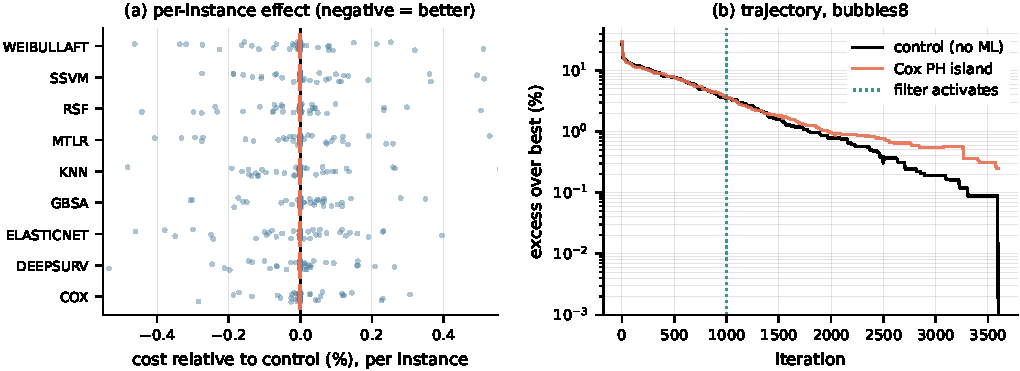
\includegraphics[width=0.95\textwidth]{figC_results.pdf}
\caption{(a) Per-instance effect of every model relative to the control over the
53 test instances. Each point is one instance and the tick marks the median; this
is the quantity the signed-rank test operates on, and it is centred on zero for
every model. (b) A representative trajectory on an instance whose runs continue
well past the activation point, so that the filter is actually operating over the
plotted window. A single ML island is shown rather than the mean of all nine:
this compares one treatment with the control without pooling distinct models.
The curve is descriptive and is not a time-to-target comparison.}

\label{fig:per-instance}
\end{figure*}

Figure~\ref{fig:per-instance}\,a shows the same result at instance resolution.
Per-instance differences include both signs, with medians near zero.
The aggregate therefore obscures variation across instances; the plot alone
does not establish symmetry of the difference distribution.

These results indicate no statistically detectable effect in \emph{either}
direction under the evaluated protocol; they do not establish equivalence.
Two models show a nominally negative degradation, but the data provide
insufficient evidence to interpret these differences as improvements.
The differences are far smaller than the between-seed variation, none approaches
significance, and the per-group breakdown shows the sign of the effect flipping
between groups for the same model: DeepSurv, for instance, records $-0.226\%$ on
the \texttt{or10} group and $+0.096\%$ on \texttt{varied}. Sign changes of this
kind are consistent with run-to-run variability.
Section~\ref{sec:diagnosis} examines potential explanations for the outcome.

\subsection{Convergence Speed}\label{sec:res-speed}

Speedups relative to the control range from $1.008$ to $1.084$, and none is
significant ($p \geq 0.15$). Two caveats limit their interpretation. First, the ten islands execute concurrently on one machine, so
per-island wall-clock times are measured under contention and a model whose
neighbours finish early is measured under lighter load than one whose neighbours
persist. Second, and more fundamentally, an iteration is not a constant unit of
work once filtering is enabled: a rejected offspring consumes an iteration
without a VND call, so an ML island performs fewer local searches per iteration
than the control by construction. Any comparison expressed per iteration
therefore uses a different computational budget. The speedups here describe
total runtime to the stopping rule, not time to a common target quality.

Figure~\ref{fig:per-instance}\,b shows a trajectory directly, with the activation
point marked; its visual proximity is descriptive, without a separate
trajectory-level hypothesis test.

Rejection rate and speedup are strongly rank-correlated across the nine models
(Spearman $\rho = \RejectionSpeedRho$, $p = \RejectionSpeedP$). Skipping VND
reduces the number of local-search calls by construction; the cross-model
association does not isolate its causal effect on wall-clock runtime. Establishing an end-to-end
benefit additionally requires considering quality and total computational cost.

\subsection{Filter Activity}\label{sec:res-activity}
% [DATA] computed from analysis_test/parsed/island_summaries.csv:
%   2385 ML island-runs; 852 (35.7%) end before iteration 1000; among the
%   remaining 1533 the median filtering window is 1083 iterations = 52% of the
%   run; mean rejections per trigger-reaching run range 72.7 (RSF) to 375.1 (COX).
% Also analysis_test/results/ml_activation.csv and training_events_summary.csv.

To interpret the absence of a statistically detectable effect, we quantify how
much filtering occurred.

Where training occurred, the trigger fired at iteration $1000$ (the budget
floor of $20\%$ of the $5000$-iteration budget), meaning the event-count
condition was already satisfied in those runs. Because the search
terminates on stagnation rather than exhausting the budget, however, not every
run reaches that point. Of the $2385$ ML island-runs, $852$ ($35.7\%$) stopped
before iteration $1000$ and therefore execute without active filtering; at the
instance level, $6$ of the $53$ instances have no recorded rejections. The
released summaries include both the full set and the 47-instance active subset.

The remaining $1533$ runs reached the trigger iteration; three stopped exactly
there with no subsequent filtering window.
The median filtering window is $1083$ iterations, or $52\%$ of the run's length,
and the mean number of offspring rejected per trigger-reaching run ranges from
$73$ for RSF to $375$ for Cox (medians $41.5$ and $211.5$). Aggregated over the experiment the filter rejected between
$12{,}653$ and $65{,}265$ offspring depending on the model, each rejection
eliminating one local-search call.

The filter was active in more than fifteen hundred runs, with a median active
window exceeding half the run length, and removed tens of thousands of offspring
from local search. No statistically significant change in quality or speed was
detected. These measurements indicate that limited activation alone is
insufficient to account for the aggregate outcome.

\subsection{Threshold Behaviour}\label{sec:res-threshold}
% [DATA] source: analysis_test/results/threshold_stability.csv
% pct_mean 82.9-85.8; obj_negative% 12.6 (COX) - 24.1 (MTLR).

Two properties of the calibrated thresholds anticipate the diagnosis.

The first is convergence. Although the percentile search ranges over
$50$--$95$ and is run independently for every model, every instance and every
seed, the selected percentile clusters tightly at $82.9$--$85.8$ across all nine
models. This concentration across heterogeneous model families suggests that the
shape of the calibration objective contributes substantially to threshold
selection.

The second is more direct. The calibration objective rewards a positive survival
gap: accepted offspring should outlive rejected ones on the held-out split.
Between $12.6\%$ (Cox) and $24.1\%$ (MTLR) of calibrations return a
\emph{negative} penalised objective. Equation~\eqref{eq:softcap} subtracts an
over-rejection penalty, so a negative objective does not necessarily imply a
negative survival gap. These frequencies describe calibration outcomes, while
Section~\ref{sec:diagnosis} measures discrimination directly. The gap uses
observed durations, including censored durations on ML islands, so it is a
calibration heuristic rather than a censoring-adjusted survival estimate.

% ============================================================================
\section{Diagnosis}\label{sec:diagnosis}
% The core of the paper. Every number below is measured; sources in comments.
% ============================================================================

Section~\ref{sec:results} found no statistically detectable effect. We examine
the tested models, representations and target, then cost-rank transmission.
Model, oracle and lineage comparisons use run-aware cross-validation.
Univariate features and partial-VND scores are direct concordance measurements.
The legacy population-feature multivariate analysis uses shuffled solution-level
folds and is exploratory. All diagnostics retain the sample-selection
limitations of Section~\ref{sec:fw-survival}.

\subsection{Discrimination Across Model Classes}\label{sec:diag-cindex}
% [DATA] sources: analysis_la_cetsp/results/oracle_ceiling.csv (PRE_geom row,
% run-aware folds) and feature_ceiling.csv (independent replication, different
% sampling). Report the run-aware numbers.

We first examine whether greater model flexibility improves discrimination on
the deployed feature set.

Establishing this required a measurement the online pipeline does not provide.
Of the nine deployed models only Cox records a concordance index during
training; the other eight persist a rejection threshold and nothing else, so
their discriminative power is invisible at run time. We therefore refitted all
nine offline on control-island logs. Diagnostic adjustments use a $0.01$
penalty for Cox and Weibull AFT, and 100 rather than 200 final-fit epochs for
neural models. The AFT diagnostic uses negative expected survival rather than
negative median survival. We evaluated these model families with
run-aware cross-validation on the five diagnostic instances
(Table~\ref{tab:cindex}).

% [DATA] source: analysis_la_cetsp/results/model_ceiling.csv (run-aware folds,
% diagnostic settings, 17568 solutions over 5 instances)
\begin{table}[htbp]
\caption{Cross-validated concordance of nine survival model families under the
diagnostic settings, using the deployed feature set and averaged over five instances spanning the structural
groups ($n = 17{,}568$ logged solutions). Chance is $0.500$. The tested models
show limited discrimination; the values are not a performance ranking.}
\label{tab:cindex}
\centering\small
\begin{tabular}{llr}
\toprule
Model & Class & $C$ \\
\midrule
RSF        & tree ensemble        & 0.544 \\
GBSA       & gradient boosting    & 0.544 \\
SSVM       & kernel / ranking     & 0.540 \\
Cox PH     & linear               & 0.537 \\
ElasticNet & penalised linear     & 0.536 \\
WeibullAFT & parametric AFT       & 0.532 \\
KNN        & non-parametric       & 0.518 \\
DeepSurv   & deep network         & 0.501 \\
MTLR       & deep network         & 0.495 \\
\bottomrule
\end{tabular}
\end{table}

% Panels (a) and (b) were separate single-column figures; as two floats they
% could not share a page with text and LaTeX gave them a float page of their own.
% Merged into one full-width float they sit at a page top and leave the rest for
% text. Section 6.2 refers to panel (b).
\begin{figure*}[!tbp]
\centering
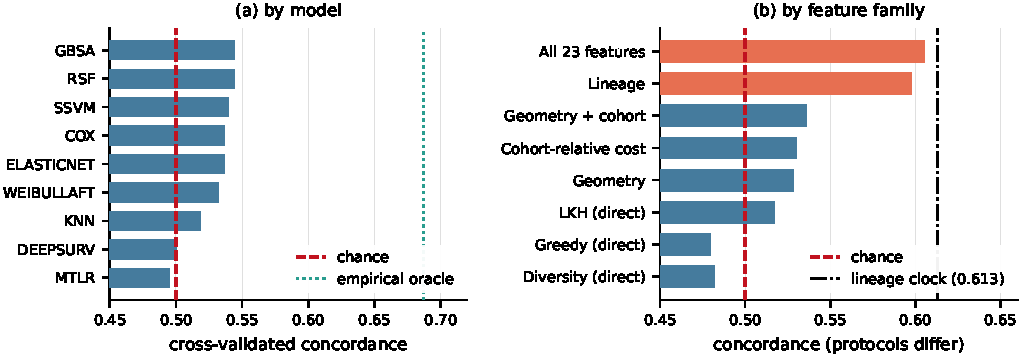
\includegraphics[width=0.95\textwidth]{figA_landscape.pdf}
\caption{The diagnostic landscape. (a) Nine model families under the diagnostic settings against the
chance level and against the empirical oracle reference of Section~\ref{sec:diag-oracle};
the spread across seven hypothesis classes is smaller than the distance from any
of them to the oracle. (b) Feature families with mixed protocols: diversity and partial-stage bars
are direct scores; the other bars use run-aware models. The dashed clock
reference applies to the lineage sample. The two highlighted bars are
measured on the shorter, drift-heavier runs described in
Section~\ref{sec:diag-features}; the
relevant comparison is with the index baseline measured on the same runs.}
\label{fig:model-landscape}
\end{figure*}

The nine models span linear, penalised linear, parametric, kernel-based,
non-parametric, tree-ensemble and deep-network hypothesis classes, and every one
of them lands between $0.495$ and $0.544$ (Figure~\ref{fig:model-landscape}). Two additional measurements on
different samples of the same log collection give nearby values: a three-model
diagnostic returns $0.532$, $0.530$ and $0.535$ for Cox, RSF and GBSA, and the
\texttt{PRE\_GEOM} row of Table~\ref{tab:oracle} agrees to within $0.013$.

The results provide no evidence of a consistent gain from greater model
flexibility under the tested settings. They motivate examining the inputs and
prediction target alongside model choice. They do not establish the best
achievable performance of other architectures or tuning strategies.

We stress that this is not a ranking of the nine models, and the differences
within the table should not be read as one. A spread of $0.049$ concordance
across nine model families, all within $0.045$ of chance, is not a basis for
recommending any of them; \citet{burk2026neutral} report in a large-scale
neutral comparison that even on genuine survival data with real signal, model
classes separate far less cleanly than the methods literature implies. What the
table supports is limited discrimination under the evaluated representations and
training protocol.

These scores describe the positive-lifetime eviction sample. Zero-lifetime
records and unlogged terminal survivors are absent. Their exclusion may change
the apparent discrimination; a low recorded censoring rate does not remove this
selection concern.

\subsection{Discrimination Across Feature Families}\label{sec:diag-features}
% [DATA] sources: feature_importance.csv, feature_prototype_univariate.csv,
% feature_prototype_multivariate.csv, diversity_signal.csv, partial_vnd_signal.csv

We next examine sensitivity to the representation. Because
features can be prototyped offline against the logged solutions without
modifying the solver or repeating any experiment, we were able to test four
representation families. These exploratory analyses use different samples and
validation protocols, as stated above.

\emph{Deployed geometry.} Taken individually, none of the ten features in
production shows substantial discrimination: every univariate concordance lies within $0.019$ of
chance, and the two centroid coordinates within $0.005$. The signs are not even
consistent across instances. Inspection explains why. Six of the ten
(the three bounding-box quantities, the two centroid coordinates and the
centroid distance sum) are effectively constant within an instance, because
every tour visits the same disks and therefore spans nearly the same region;
and mean edge length is related to pre-VND tour cost, although its
implementation omits the closing edge.

\emph{Population-relative cost.} The eviction rule ranks an individual against
the current population, so scale-free relative quantities are a more principled
choice than absolute geometry: the percentile of an offspring's pre-VND cost
within the cohort alive at its birth, its ratio to the cohort median and
minimum, its $z$-score, and its ratio to the running best. Multivariate
concordance over this family reaches $0.529$--$0.542$.

\emph{Diversity.} Survival is governed by value rank \emph{and} distance rank,
so we examined a proxy: directed Chamfer distance between pre-VND point sets,
using at most 80 points per tour and 15 recorded cohort members. Mean and minimum
distances have direct concordances $0.478$ and $0.482$. These raw feature scores
may have a protective direction below $0.5$; they do not directly test the
solver's edit-distance criterion.

\emph{Partial local search.} Finally we tested whether a cheap prefix of the
pipeline provides survival discrimination: we scored recorded costs after
the greedy stage and after LKH. No early-exit policy was deployed in this probe. The corresponding concordances are
$0.479$ and $0.517$; the completed VND cost reaches $0.651$, by which point the expense the
filter exists to avoid has already been incurred.

\emph{Lineage.} The four families above all describe the offspring itself, and
so must survive the local search to be useful. The remaining family describes
where it \emph{came from}, and does not pass through the local search at all:
the cost and fitness of both parents, which are population members that have
already been evaluated; the two offspring-to-parent edit distances measured before mutation; and whether mutation fired. ``Offspring of two
strong, mutually distant parents'' is a prior on offspring quality that no
geometric descriptor can express. This family could not be prototyped from the
existing logs, since parent identity was not recorded, so we instrumented the
solver and re-ran the affected instances to obtain it.

% [DATA] source: analysis_la_cetsp/results/lineage_signal.csv, 4 instances,
% 4902 solutions, run-aware folds. Best-of-three-models column:
%   PRE_all 0.588 | LINEAGE 0.598 | PRE+LINEAGE 0.605 | DRIFT 0.613
Lineage features score $0.598$ on their own and $0.605$ combined with
everything else. On the same data the birth iteration \emph{alone} scores
$0.613$. Twenty-three combined features (geometry, relative cost and lineage), fitted by
three model classes, do not beat a single integer recording when the offspring
was created. (Absolute levels are elevated here relative to
Table~\ref{tab:cindex} because these runs are short and therefore drift-heavy;
the comparison against the drift control, not the level, is what carries the
conclusion.)

This comparison illustrates the role of the drift control: an apparent increase
from $0.53$ to $0.60$ across different samples does not by itself establish more
useful predictive information. We recommend a time-index baseline for feature
evaluations on improving search trajectories and return to this in
Section~\ref{sec:gate}.

The tested representations show limited discrimination on their recorded
samples. The oracle and lineage experiments include matched drift controls;
there is no matched clock comparison for every exploratory family. These
findings motivate examining the target and recorded post-step information
(Figure~\ref{fig:model-landscape}\,b).

\subsection{An Empirical Oracle Reference}\label{sec:diag-oracle}
% [DATA] source: analysis_la_cetsp/results/oracle_ceiling.csv (run 2026-08-18)
% Folds are GROUP-AWARE (GroupKFold by run). This matters: with plain KFold the
% same run appears in train and test, and on bonus1000 that inflated RSF on the
% PRE_geom set from 0.512 to 0.660 — pure run-identity leakage. Report the
% group-aware numbers and state the protocol explicitly; a reviewer replicating
% with naive CV would otherwise get a different answer.

\begin{table}[htbp]
\caption{Empirical oracle reference. Concordance averaged after taking the best of Cox, RSF and GBSA within each
instance (run-aware folds; optimistic model selection) over five instances spanning the structural groups. ORACLE
receives recorded post-VND information, unavailable to a filter that skips VND.
Its fitted performance is a diagnostic reference rather than a formal upper bound.}
\label{tab:oracle}
\centering\small
\begin{tabular}{llr}
\toprule
Feature set & Information used & $C$ \\
\midrule
% \textsc here triggered "Font shape T1/cmss/m/sc not available": the CAS class
% sets tables in a sans family with no small-caps shape at 9pt. \texttt exists in
% every family and reads the same way for these identifiers.
\texttt{PRE\_GEOM}   & deployed geometry     & 0.529 \\
\texttt{PRE\_POP}    & cohort-relative cost  & 0.530 \\
\texttt{PRE\_ALL}    & best legitimate set   & 0.536 \\
\texttt{DRIFT}       & birth iteration only  & 0.536 \\
\midrule
\texttt{ORACLE}      & post-VND outcome      & \textbf{0.687} \\
\texttt{ORACLE\_ALL} & oracle $+$ all pre-VND & \textbf{0.688} \\
\bottomrule
\end{tabular}
\end{table}

To examine the target, a model is given recorded \emph{post}-VND information
(the cost VND actually produced, that cost's rank within the cohort alive at the
offspring's birth, and the relative gain VND delivered), none of which a real
filter can observe, since obtaining them requires running the very local search
the filter exists to skip. This oracle provides an empirical reference for
survival prediction with additional information. A fitted model on these
descriptors does not establish a universal upper bound for all pre-VND predictors.

Table~\ref{tab:oracle} gives the result, and it supports three conclusions.

\emph{Recorded post-VND information improves discrimination.} The oracle reaches
$C = 0.687$, above the tested pre-VND representations but below perfect
prediction. Survival depends on subsequent population changes: an offspring is
evicted as better or more diverse individuals accumulate around it. These future
events are not directly observed at birth, although their effects may be partly
predictable. The result motivates considering target uncertainty alongside
representation and model limitations.

\emph{Pre-VND features add little in this evaluation.} Augmenting the oracle with
every pre-VND feature we engineered moves the score from $0.687$ to $0.688$.
This small observed increment suggests limited additional predictive value under
the tested protocol; it does not establish conditional independence.

\emph{The pre-VND features match the drift reference.} A relevant result in the
table is the equality of \texttt{PRE\_ALL} ($0.536$) and \texttt{DRIFT}
($0.536$). The best legitimate feature set we could construct (ten geometric
descriptors plus four population-relative cost statistics, over five instances)
matches the birth-iteration baseline. This suggests that part of the apparent
predictive performance reflects search progress. Such pooled discrimination does
not establish an ability to distinguish contemporaneous candidates, which is
the relevant comparison for filtering.

One limitation should be stated plainly. Survival is governed by
$\textit{fitness} = \textit{value\_rank} + \beta \cdot \textit{distance\_rank}$.
Neither population rank is exactly reconstructible. Unlogged or unsampled
live members are absent, and the cost statistics describe the recorded cohort.
For distance rank, edit distance is computed after VND against the
current population, and only pre-VND coordinates are recorded. The oracle thus
uses an incomplete description of the post-VND state. Its measured performance
may understate what a richer model and fuller information could achieve, which
limits the conclusions that can be drawn from this check alone.

\subsection{Cost-Rank Transmission Through Local Search}\label{sec:diag-stages}
% [DATA] source: analysis_la_cetsp/results/rank_transmission.csv (2026-09-02)
% NOTE: the stage-by-stage correlations previously appeared here as a
% full-width table as well as on the arrows of Figure~\ref{fig:rank-chain}.
% That duplicated the same six numbers in two full-width floats. The table was
% removed; the end-to-end rows it also carried are stated in the text below,
% which is where they are argued anyway.
\begin{table}[htbp]
\caption{End-to-end correlation between pre- and post-local-search cost
ordering in recorded positive-lifetime solutions. The cohort column correlates
percentiles within reconstructed recorded cohorts; it does not recover the full
live population or restrict every scored pair to the same birth time.
Stage-by-stage values are given on Figure~\ref{fig:rank-chain}.}
\label{tab:stage-chain}
\centering\small
\begin{tabular}{lrr}
\toprule
Instance & pooled & cohort percentile \\
\midrule
% Generated by tools/export_paper_results.py
concentricCircles4 & $+0.48$ & $+0.15$ \\
kroD100\_or2 & $+0.13$ & $+0.08$ \\
rat195\_or30 & $+0.48$ & $+0.21$ \\
\bottomrule

\end{tabular}
\end{table}
The oracle analysis of Section~\ref{sec:diag-oracle} addresses prediction of the
label. To examine the transformation of pre-VND cost information, we instrumented the local
search to record the tour cost after each of its internal stages, and tracked
how the ordering of offspring propagates through the pipeline
(Figure~\ref{fig:rank-chain} and Table~\ref{tab:stage-chain}).

\begin{figure*}[!tbp]
\centering
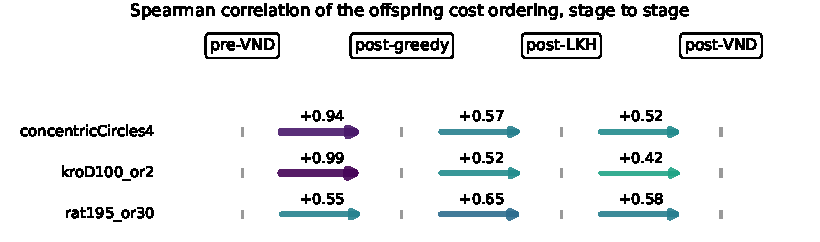
\includegraphics[width=0.86\textwidth]{fig3_rank_chain.pdf}
\caption{Propagation of the offspring cost ordering through the local-search
pipeline. Arrow thickness and colour encode the Spearman correlation between the
ordering entering and leaving each stage. Transmission varies by stage and
instance; substantial greedy-stage preservation occurs on two of the three.}
\label{fig:rank-chain}
\end{figure*}

Rank transmission varies by stage and instance (Figure~\ref{fig:rank-chain}).
Greedy-stage correlations span $\GreedyMin$--$\GreedyMax$; the two larger values
show substantial preservation, while the third is already attenuated. LKH-stage
correlations span $\LkhRankMin$--$\LkhRankMax$, and the closing stages span
$\RefineMin$--$\RefineMax$. This identifies several potential sources of rank
attenuation rather than a single universal loss point.

Pooled pre/post correlations span $\GlobalRankMin$--$\GlobalRankMax$; correlations
of recorded-cohort percentiles span $\CohortRankMin$--$\CohortRankMax$.
The latter adjusts for relative standing at birth but still pools observations
over time and uses incomplete cohorts. It is a temporal diagnostic, not proof
that all search-phase drift has been removed.

\subsection{Rank--Gain Association Within Local Search}\label{sec:diag-contraction}
% [DATA] source: analysis_la_cetsp/lkh_character.py, which now writes
% results/contraction_kappa.csv; make_figures.py reads that file for the panel
% titles of Figure~\ref{fig:contraction}, so the two can no longer disagree.
%
% The table that used to stand here listed exactly the three kappa values that
% the figure prints in its panel titles. It was removed for two reasons: it was
% a redundant float in the most float-dense part of the paper, and because it
% was transcribed by hand from console output while the figure recomputed the
% same quantity with a different estimator, the two had silently drifted apart
% on two of the three instances. One source of truth now: the CSV.
Figure~\ref{fig:contraction} examines a mechanism consistent with this
attenuation. For each offspring we measured its cost
rank within its recorded cohort at birth, and the relative improvement LKH
then delivered. The two are positively rank-correlated: the contraction
coefficient $\kappa_{\mathrm{LKH}}$ (the Spearman correlation between those two quantities,
computed within each run and averaged across runs) is $\LkhCircle$, $\LkhKro$ and $\LkhRat$ on the three instances. Lower-ranked inputs tend to receive larger
relative LKH improvements.

\begin{figure*}[!tbp]
\centering
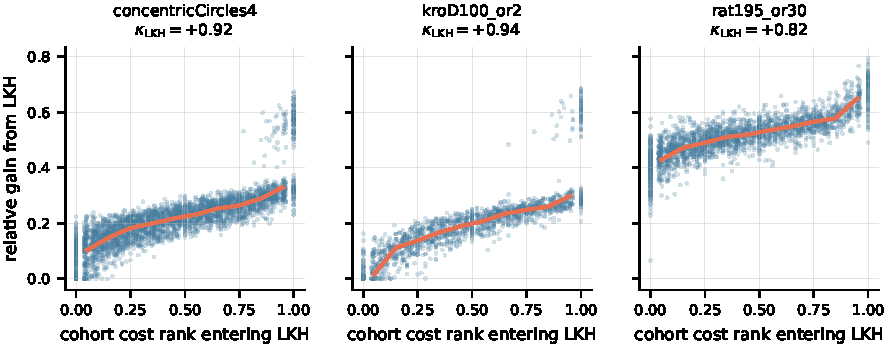
\includegraphics[width=0.92\textwidth]{fig4_contraction.pdf}
\caption{LKH rank--gain association. Each point is one recorded offspring: its
post-greedy cost percentile within its recorded birth cohort, against the relative improvement LKH
returned. The line is the binned median. Its upward trend indicates larger gains
for lower-ranked inputs; rank preservation also depends on the gain magnitudes
and their variation. Each panel is titled with the contraction
coefficient $\kappa_{\mathrm{LKH}}$, the Spearman correlation between the two plotted
quantities, computed within each run and averaged across runs.}
\label{fig:contraction}
\end{figure*}

This pattern is consistent with compensatory improvement
(Figure~\ref{fig:contraction}): lower-ranked inputs tend to receive larger
relative gains. Together with the stage-wise correlations, it suggests a
mechanism for attenuation of entering cost order. Rank--gain association alone
does not measure a reduction in the spread of costs.

These measurements are consistent with the limited discrimination observed
across the tested models and pre-VND feature families, the small increment from
adding those features to the oracle, and the contribution of temporal drift to
pooled correlations. They do not establish that all predictive information in
the pre-VND state is absent. In particular, a rank--gain correlation alone does
not determine post-step rank preservation or the usefulness of other descriptors.

The practical implication is to assess rank transmission and predictive value
before investing further in a filtering design. In the evaluated system, their
joint evidence supports reconsidering pre-VND survival filtering. This motivates
the one-sided screening procedure in the next section.


% ============================================================================
\section{A Viability Gate for Pre-Local-Search Filtering}\label{sec:gate}
% ============================================================================

The diagnosis of Section~\ref{sec:diagnosis} is specific to our system, but the
way it was reached is not. Each step measured a property of the pipeline rather
than of the surrogate, and every one of those measurements could have been taken
\emph{before} the surrogate existed. This section states them as a reusable
screening procedure, calibrates the central one, and applies the result
retrospectively to our own project.

\subsection{Three Checks}\label{sec:gate-checks}

The procedure comprises three measurements, each addressing a potential
constraint on pre-local-search filtering. They use instrumented logs and offline
fits, with enough independent runs for run-aware validation.

\textbf{Check 1: Is the label reachable?} Fit a model on information that is
available only \emph{after} the expensive step, and measure how well it predicts
the intended target. This is the empirical oracle of
Section~\ref{sec:diag-oracle}. Limited discrimination even with post-step
information motivates reassessing the target, representation and available data.
Its interpretation depends on the completeness of that information and the
fitted models; it is not a formal upper bound for all pre-step predictors.

\textbf{Check 2: Does the pipeline preserve the ordering?} Instrument the
expensive step to record its input and output cost, and compute the
\emph{contraction coefficient}
\begin{equation}
\kappa \;=\; \rho_{s}\bigl(r_{\text{in}},\; g\bigr),
\label{eq:kappa}
\end{equation}
where $\rho_s$ is Spearman's rank correlation, $r_{\text{in}}$ is a candidate's
cost percentile within the reconstructed recorded cohort at its birth,
and $g$ is the relative improvement of that same step. We distinguish
$\kappa_{\mathrm{LKH}}$ (post-greedy to post-LKH) from
$\kappa_{\mathrm{VND}}$ (pre-VND to final VND). As $\kappa \to 1$,
lower-ranked inputs tend to receive larger relative gains. Whether these gains
substantially alter the output ordering also depends on their magnitudes and
the input costs. Interpret $\kappa$ alongside direct input--output rank
correlations and a calibration for the pipeline under study.

\textbf{Check 3: Does the feature set beat the clock?} Evaluate any candidate
representation against a baseline consisting of the iteration index alone. Data
generated by an improving search carries a strong temporal trend, and any feature
correlated with time may appear predictive in a pooled evaluation without
distinguishing contemporaneous candidates. A gain over the clock is a reason for
further within-cohort and deployment evaluation, rather than proof of benefit.
The lineage family of
Section~\ref{sec:diag-features} scored $0.598$, while its matched iteration-index
baseline scored $0.613$. Comparisons across different samples are exploratory.

\subsection{Calibrating the Coefficient}\label{sec:gate-curve}

We examine full-VND rank--gain dependence on 25 diagnostic instances. For each,
we use up to three recent runs and the last 800 records in numeric file order,
retaining positive-lifetime records and at least three recorded cohort peers.
Selected runs, counts and input hashes are released. Cohorts are incomplete;
original membership is held fixed throughout this sensitivity experiment.

For each of eleven nominal dependence settings, a Gaussian copula reassigns the
observed gains among candidates with valid pre-step cohort percentiles. Five
reassignments are drawn per run using seed zero; other gains stay fixed. The gain
multiset is preserved, while $q'_i=p_i(1-g'_i)$. Ties and finite samples mean the
realised $\kappa_{\mathrm{VND}}$ need not equal its nominal setting, so both are
reported. This does not simulate new survival trajectories or filtering.

Cost-rank concordance $C_{\mathrm{rank}}$ is computed directly over pairs with
distinct output percentiles: agreeing input order receives one, tied input
order one half, and reversed input order zero. Output ties are excluded. This
score differs from rescaled Kendall $\tau_b$ and from survival concordance.
Results are averaged over repeats and runs, then equally across instances.

\begin{table}[htbp]
\caption{Full-VND sensitivity analysis on recorded cohorts. The first column is
nominal dependence; the second is mean realised $\kappa_{\mathrm{VND}}$.
The final columns report mean cost-rank concordance and between-instance SD.}
\label{tab:kappa-curve}
\centering\small
\begin{tabular}{rrrr}
\toprule
Nominal & Realised & $C_{\mathrm{rank}}$ & SD \\
\midrule
% Generated by tools/export_paper_results.py
0.00 & -0.001 & 0.730 & 0.010 \\
0.10 & 0.095 & 0.713 & 0.008 \\
0.20 & 0.199 & 0.693 & 0.010 \\
0.30 & 0.295 & 0.675 & 0.011 \\
0.40 & 0.391 & 0.656 & 0.012 \\
0.50 & 0.495 & 0.635 & 0.012 \\
0.60 & 0.596 & 0.613 & 0.014 \\
0.70 & 0.695 & 0.590 & 0.015 \\
0.80 & 0.800 & 0.560 & 0.019 \\
0.90 & 0.901 & 0.526 & 0.022 \\
0.95 & 0.950 & 0.502 & 0.026 \\
\bottomrule

\end{tabular}
\end{table}

\begin{figure*}[!tbp]
\centering
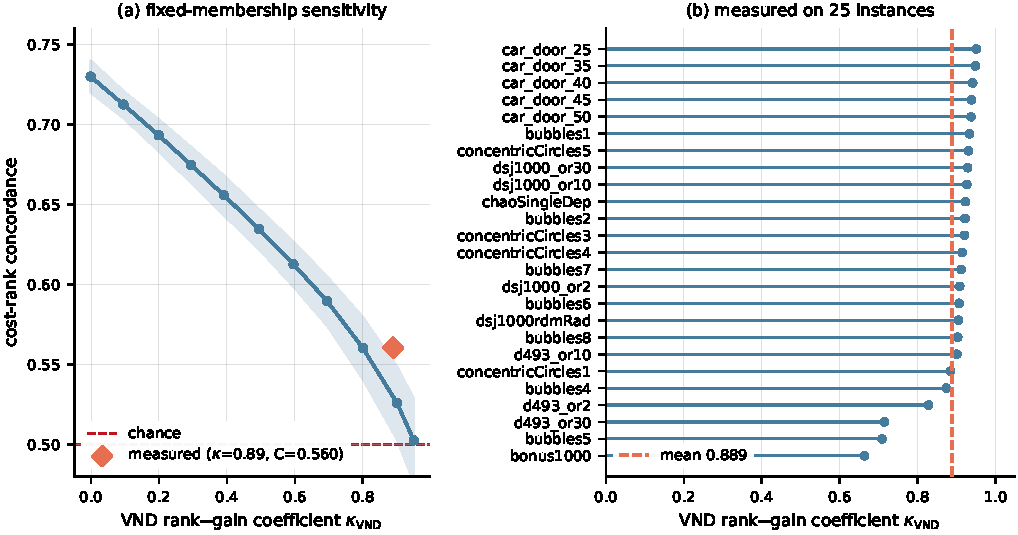
\includegraphics[width=0.95\textwidth]{figB_kappa.pdf}
\caption{(a) Cost-rank concordance versus mean realised full-VND rank--gain
coefficient. The band is one SD across instances; the diamond marks observed
data. (b) Observed coefficients across the 25 diagnostic instances, including
eight development instances. This is a conditional sensitivity analysis, not
a universal viability threshold.}
\label{fig:kappa-curve}
\end{figure*}

Table~\ref{tab:kappa-curve} and Figure~\ref{fig:kappa-curve} show decreasing
rank concordance as dependence increases under the specified reassignments.
The observed mean is $\kappa_{\mathrm{VND}}=\KappaVNDMean$, with
$C_{\mathrm{rank}}=\ObservedRankC$. At the nominal zero setting, mean
concordance is $\CalibrationStartC$; at the largest setting it is
$\CalibrationEndC$. Zero rank--gain correlation does not imply perfect order
preservation, since individual gains still vary.

The observed point need not lie on the synthetic curve: the copula changes
dependence beyond a single correlation, and the fixed recorded membership omits
feedback through survival. We therefore make no calibrated-performance guarantee.
The oracle's survival concordance of $0.687$ is a separate diagnostic of a
different target and cannot validate this cost-rank curve.

\subsection{The Gate Applied Retrospectively}\label{sec:gate-applied}

Table~\ref{tab:gate} applies the three checks to our project. Taken together,
the limited oracle discrimination, strong rank attenuation and lack of a feature
advantage over drift support a decision against further deployment of the tested
design. These measurements could have preceded full framework development.

\begin{table}[htbp]
\caption{The gate applied to the system of Section~\ref{sec:framework}. Check~1
is the empirical oracle of Section~\ref{sec:diag-oracle}; check~2 is
Equation~\eqref{eq:kappa} for full VND, averaged over 25 instances; check~3 compares the best
tested pre-VND feature set against the iteration index alone. The checks are
interpreted jointly for this design, without universal pass/fail cut-points.}
\label{tab:gate}
\centering\small
\begin{tabular}{lr}
\toprule
Check & Value \\
\midrule
1. Oracle concordance      & 0.687 \\
2. VND $\kappa$           & $\KappaVNDMean$ \\
3. Features / clock        & 0.605 / 0.613 \\
\bottomrule
\end{tabular}
\end{table}

Across the 25 diagnostic instances, $\kappa_{\mathrm{VND}}$ ranges from
$\KappaVNDMin$ to $\KappaVNDMax$, with mean $\KappaVNDMean$.
These values summarise recorded-cohort rank--gain association in the selected
runs, not an intrinsic constant of the problem or operator.

The checks can precede deployment of an online filtering framework. They require
instrumented logs and offline analysis, including sufficient independent runs
for model validation; one run alone cannot support run-aware cross-validation.
The present application is retrospective and exploratory. A prospective study
must specify its practical quality tolerance and computational costs before
using these measurements to make a deployment decision.

\subsection{Interpreting the Outcome}\label{sec:gate-interpret}

\textbf{The gate is one-sided.} Adverse findings across the checks can support
a decision not to proceed with a particular filtering design under the assessed
conditions. High $\kappa$, interpreted with weak input--output rank transmission
and limited predictive value, provides evidence for that decision; high
$\kappa$ alone is not an impossibility result. Favourable findings permit
further evaluation but do not establish net benefit. A low $\kappa$ addresses
only one potential obstacle, leaving target predictability, discrimination
beyond drift, calibration, overhead and search-quality effects to be assessed.
The gate therefore screens deployment choices rather than proving a universal
boundary between feasible and infeasible filtering.

We state our own values as a single calibration point rather than as a standard,
and recommend that studies of surrogate-assisted local-search filtering report
$\kappa$ alongside their outcome. One point does not determine a curve; a
literature that reports the coefficient would.

\subsection{Alternatives Suggested by the Gate}\label{sec:gate-alternatives}

The diagnostics also suggest alternative designs to evaluate, each addressing
a different potential limitation.

\emph{Consider a different target.} Attenuation of solution-quality ordering
does not by itself determine the predictability of local-search runtime. If
runtime varies substantially and is predictable from pre-step descriptors, the
architecture could support cost-aware triage. Its savings and effects on solution
quality would need separate evaluation; we did not pursue this direction here.

\emph{Move the decision point.} The gate evaluates one specific insertion:
before the expensive step. A surrogate may still earn its place elsewhere in the
loop, for example in operator or parameter selection, where the quantity being
predicted is not mediated by a contraction.

\emph{Assess alternative local-search operators.} The measured $\kappa$ depends
on the operator and the input distribution. Operators with stronger rank
preservation may provide more favourable conditions for filtering, subject to
the other checks and an end-to-end assessment.

% ============================================================================
\section{Discussion}\label{sec:discussion}
% ============================================================================

\subsection{Scope of the Findings}\label{sec:disc-scope}

Three findings define the scope of the study. The evaluated pre-local-search
survival filters show no statistically detectable benefit; the diagnostic
measurements identify limited discrimination and attenuation of cost ordering
as plausible contributing factors; and these properties can be measured before
deployment. The findings concern the tested pipeline, representations and
protocol. The transferable contribution is a screening procedure whose
interpretation requires evidence from each new setting.

The value of reporting it lies in that specificity.
\citet{pang2022counterintuitive} argue, from a different corner of evolutionary
computation, that results which contradict the field's working intuitions are
worth publishing precisely because they expose assumptions that otherwise remain
untested, and that such results are informative only when their cause is
identified rather than merely observed. The assumption exposed here is that an
offspring's pre-local-search description carries usable information about its
post-local-search fate. That assumption is implicit in every pre-local-search
filter, including our own earlier one. Explicitly measuring it helps distinguish
predictive limitations from implementation and evaluation effects.

\subsection{When Can Pre-Local-Search Filtering Pay Off?}\label{sec:disc-when}

The diagnosis suggests conditions worth evaluating, consistent with the
permissive interpretation of passing the gate.

A rank-preserving operator may retain information useful to a pre-step predictor.
The greedy stage in our sample shows substantial preservation on two instances
and weaker transmission on the third. Stronger preservation removes one concern,
while leaving the relation between cost, survival and useful rejection decisions
to be tested.

If the dominant expense is objective evaluation rather than an intervening
improvement operator, the specific rank-transmission concern may be less
relevant. Predictive accuracy and the balance between saved computation and
search-quality effects would still require evaluation.

An alternative target is local-search runtime. The measured attenuation of
quality ordering does not establish whether runtime is predictable. A model of
expected expense could support cost-aware decisions, provided its overhead and
effects on solution quality are assessed. Our logs do not record per-offspring
local-search time, so this remains a direction for future work.

\subsection{Relation to the Preliminary Study}\label{sec:disc-prelim}

The preliminary study~\citep{balemir2026lacetsp} reported that 13--26\% of
offspring could be pruned at negligible cost in quality. The present experiment
does not provide statistical support for a benefit under the larger evaluation
protocol. The shared framework makes the differences in evaluation design
relevant to interpreting the two results.

Three features of the earlier design limit interpretation. It used
four instances at a 500-iteration budget with five runs each, providing limited
evidence for separating a filtering effect from seed variance. It had no
in-run control: the filtered and unfiltered configurations were separate
executions rather than concurrent islands of the same run, so the comparison
absorbed any difference in machine state, and the reported figures were
best-of-five rather than paired. And it compared configurations per iteration
while pruning changes what an iteration costs: a filtered run performs fewer
local searches per iteration by construction, so equal-iteration comparisons
favour the filtered configuration.

That study also reported no concordance index for any fitted model, leaving the
selectivity of its pruning unresolved. The present near-chance measurements
motivate this diagnostic, but do not retrospectively determine the unmeasured
concordance of the earlier runs. The gate of Section~\ref{sec:gate} is intended
to make such an assessment part of the evaluation before deployment.

\subsection{Threats to Validity}\label{sec:disc-threats}

\emph{Unpaired seeds.} Island $i$ draws seed $\sigma + i$, so a model and the
control never share a random stream and per-instance differences contain seed
variance as well as treatment effect. Aggregation over 53 instances recovers
power, and the signed-rank test pairs at the instance level, but a paired-seed
design would have been stronger and we recommend it.

\emph{Contended timing.} All ten islands occupy one machine concurrently.
Wall-clock speedups are therefore measured under mutual load and should be read
as total-runtime comparisons under contention, as noted in
Section~\ref{sec:setup-measures}.

\emph{Breadth of the diagnosis.} The measurements are not uniformly broad. The
null result covers all 53 test instances; the contraction coefficient is measured
on 25; the concordance and oracle analyses use five instances chosen to span the
structural groups; and the stage-wise chain uses the three instances for which
the local search was instrumented. The narrowest of these, the stage chain, is
also the most mechanistic, and the wider $\kappa$ measurement is consistent with
it everywhere.

\emph{Selected records and incomplete cohorts.} Unadmitted offspring, terminal
survivors and zero-lifetime records are absent from the diagnostic sample.
Reconstructing cohorts from subsets of logs also omits live members. Neither
the cost rank nor the edit-distance rank in Equation~\eqref{eq:fitness} is
exactly reconstructed. The oracle value $0.687$ is therefore an empirical result
on this selected sample, not a ceiling for all offspring. Correcting this
selection requires recording all admission outcomes, complete population state
and terminal censoring, then repeating the diagnostic analyses.

\emph{Diagnostic comparisons.} Model/oracle and lineage experiments include
matched time-index controls, but the exploratory diversity and partial-stage
measurements do not establish incremental value beyond drift. Surpassing or
matching the clock alone does not establish conditional independence or useful
within-time discrimination. A time-only versus time-plus-features comparison
and within-time evaluation would be needed for that stronger claim.

\emph{Missing pruning ablation.} The experiment compares learned filtering with
no filtering, not with matched-rate random pruning. It therefore does not
separate the value of learned selection from the effect of reducing VND calls.
Such an ablation and time-to-target comparisons are needed to assess selective
filtering utility more directly.

\emph{One local-search design.} Every measurement concerns a single improvement
pipeline. The observed rank--gain association motivates assessment in other
settings, but does not establish its prevalence across improvement operators.
The gate has been applied retrospectively in one system without a demonstrated
successful filtering case. Prospective evaluations across operators are needed
to assess its screening value, using $\kappa$ alongside rank transmission and
end-to-end outcomes.

\emph{Logging integrity.} The parallel islands write to a shared standard output
without a lock, so a small fraction of log lines interleave and yield
uninterpretable iteration numbers. These are discarded by range filtering before
analysis. The defect affects log presentation only, not the search itself.

% ============================================================================
\section{Conclusion}\label{sec:conclusion}

We built a complete survival-based offspring filter for a state-of-the-art
memetic algorithm for the CETSP: nine survival models, an adaptive training
trigger grounded in events-per-variable, validation-calibrated rejection
thresholds, a runtime rejection cap, a resident-process inference path that
removes the cross-language latency identified as the main obstacle in earlier
work, and a parallel harness that places all nine treatments and an unfiltered
control in the same run. Evaluated on 53 benchmark instances with five seeds, the
filter changes neither solution quality nor convergence speed to any
statistically detectable degree, in either direction.

The diagnostic contribution is a set of measurements that helps interpret this
outcome. The tested models show limited survival discrimination, while the
tested representations show limited discrimination. The oracle and lineage
comparisons provide matched iteration-index controls. A model using recorded post-local-search information
reaches $0.687$, an empirical reference rather than a formal upper bound.
Local search attenuates entering cost ordering, with a rank correlation between
recorded cohort position and full-VND gain of $\KappaVNDMean$ averaged over
25 instances. This provides a plausible mechanism for the limited usefulness
of cost-based pre-VND descriptors in the evaluated pipeline.

These findings motivate a one-sided viability gate comprising three diagnostic
checks that can precede full surrogate deployment. The contraction coefficient
is calibrated against cost-rank concordance on the observed data, and interpreted
alongside target predictability and discrimination beyond temporal drift.
Applied retrospectively, the joint evidence supports a decision against further
deployment of the tested design. Passing the gate would instead justify further
evaluation; it would not establish net benefit. The procedure supplies neither
a universal cut-point nor an impossibility claim for other filtering designs.

Three directions follow: assess local-search runtime as a target for cost-aware
triage, including its effects on solution quality; evaluate the gate prospectively
across different improvement operators; and examine surrogate decisions elsewhere
in the search loop. Each requires direct evidence of predictive usefulness and
end-to-end benefit.

Code, parsed results and analysis scripts accompany the paper; raw logs are
available on request as detailed in the data-availability statement.
% ============================================================================

% ============================================================================
% HIGHLIGHTS — submitted to ESWA as a separate file, 3-5 bullets, <=85 chars each.
% Keep each highlight under 85 characters when editing.
%
%   Nine survival filters show no significant quality or speed difference
%   Matched clock controls contextualise oracle and lineage discrimination
%   Local search attenuates offspring cost ordering in the tested pipeline
%   A one-sided viability gate supports screening before surrogate deployment
%   Passing the gate permits further evaluation without establishing benefit
%
% GRAPHICAL ABSTRACT — fig3_rank_chain.pdf is the natural candidate: it states
% the mechanism in one image without needing the paper's vocabulary.
% ============================================================================

\section*{CRediT authorship contribution statement}
\textbf{Demir Balemir}: Conceptualisation, Methodology, Software,
Formal analysis, Investigation, Data curation, Visualisation,
Writing -- original draft.
\textbf{Deniz Cant{\"u}rk}: Conceptualisation, Supervision, Validation,
Writing -- review and editing.

\section*{Declaration of competing interest}
The authors declare that they have no known competing financial interests or
personal relationships that could have appeared to influence the work reported
in this paper.

\section*{Data availability}
% NOTE: the raw per-solution logs are ~3.4 million JSON files totalling roughly
% 17 GB, which cannot be hosted on the code repository. The wording below is
% deliberately precise about what is and is not released. If the logs are later
% deposited (Zenodo or similar), add the DOI here and widen the claim.
The solver, survival-modelling pipeline, diagnostic scripts and retained
measurement CSVs are publicly available at
\url{https://github.com/DemirBalemir/MA-CETSP-ml-optimization}, together with
parsed end-to-end results. The release rebuilds tables and figures from these
retained measurements and documents their evaluation protocols. Raw per-solution
logs, approximately 3.4 million records, are available from the authors on request
for recalculating diagnostics. The full-VND calibration includes a run manifest
and input hashes; exact historical selections for every older probe are not
bundled. The repository README distinguishes result-level reproduction from
refitting models on the original logs.

\section*{Declaration of generative AI and AI-assisted technologies in the
manuscript preparation process}
During the preparation of this work, the authors used ChatGPT and Codex (OpenAI)
and Claude (Anthropic) to assist with developing and reviewing analysis code,
generating and checking tables and figures, and drafting and editing portions of
the manuscript. The authors reviewed and edited the output as needed and take
full responsibility for the content of the published article.

\printbibliography

\end{document}
